% Báo cáo bài tập lớn — Tư vấn và triển khai hệ thống Smart Parking IoT trên AWS
% Biên dịch:  cd report && latexmk -pdf main.tex      (pdflatex + gói vntex)
\documentclass[a4paper,oneside]{report}
\usepackage[fontsize=13pt]{scrextend}

% ─── Thông tin cần điền (sửa một lần ở đây) ───────────────────────────────
\newcommand{\Truong}{TRƯỜNG ĐẠI HỌC CÔNG NGHỆ}
\newcommand{\Khoa}{KHOA CÔNG NGHỆ THÔNG TIN}
\newcommand{\HocPhan}{Điện toán đám mây}
\newcommand{\MaLop}{INT3319E\_2}
\newcommand{\GVHD}{Nguyễn Ngọc Tân}
\newcommand{\NoiNam}{HÀ NỘI -- 2026}
\newcommand{\TenDeTai}{HỆ THỐNG BÃI ĐỖ XE THÔNG MINH (SMART PARKING) TRÊN NỀN TẢNG ĐIỆN TOÁN ĐÁM MÂY AWS}

% ─── Gói và định dạng ─────────────────────────────────────────────────────
\usepackage[T5]{fontenc}
\usepackage[utf8]{inputenc}
\usepackage[vietnamese]{babel}
\usepackage{mathptmx}                 % Times
\usepackage[scaled=0.92]{helvet}
\usepackage{courier}
\usepackage[left=3cm,right=2cm,top=2.5cm,bottom=2.5cm]{geometry}
\usepackage{setspace}\setstretch{1.3}
\usepackage[table]{xcolor}
\usepackage{graphicx,float,array,booktabs,longtable,tabularx,multirow,makecell}
\usepackage{enumitem}\setlist{itemsep=2pt,topsep=4pt}
\usepackage{caption}\captionsetup{font=small,labelfont=bf}
\usepackage{fancyhdr}
\usepackage{titlesec}
\usepackage{tikz}
\usetikzlibrary{positioning,arrows.meta,shapes.geometric,fit,calc,backgrounds,babel}
\usepackage{fvextra}
\usepackage[most]{tcolorbox}
\newcommand{\enquote}[1]{\textquotedblleft #1\textquotedblright}
\usepackage{amssymb}
\usepackage[hidelinks,unicode]{hyperref}
\usepackage{bookmark}

\definecolor{aws}{HTML}{FF9900}
\definecolor{navy}{HTML}{232F3E}
\definecolor{edge}{HTML}{2E7D32}
\definecolor{web}{HTML}{1565C0}
\definecolor{soft}{HTML}{F4F6F8}
\definecolor{todo}{HTML}{C62828}

% Ô cần điền: in màu đỏ để dễ tìm
\newcommand{\dien}[1]{\textcolor{todo}{[#1]}}
\newcommand{\code}[1]{\texttt{\small #1}}

\titleformat{\chapter}[display]{\bfseries\Large\centering}{CHƯƠNG \thechapter}{6pt}{\Large\MakeUppercase}
\titlespacing*{\chapter}{0pt}{-10pt}{18pt}
\titleformat{\section}{\bfseries\large}{\thesection}{0.6em}{}
\titleformat{\subsection}{\bfseries\normalsize}{\thesubsection}{0.6em}{}
\setcounter{secnumdepth}{3}
\setcounter{tocdepth}{2}

\pagestyle{fancy}
\fancyhf{}
\fancyfoot[C]{\thepage}
\renewcommand{\headrulewidth}{0pt}
\fancypagestyle{plain}{\fancyhf{}\fancyfoot[C]{\thepage}\renewcommand{\headrulewidth}{0pt}}

\DefineVerbatimEnvironment{lenh}{Verbatim}{fontsize=\footnotesize,breaklines,frame=single,framesep=6pt,rulecolor=\color{gray!50},xleftmargin=4pt}

\newtcolorbox{ghichu}[1][Ghi chú]{colback=soft,colframe=navy!70,fonttitle=\bfseries\small,title=#1,boxrule=0.5pt,arc=2pt,left=6pt,right=6pt}

\renewcommand{\arraystretch}{1.25}
\setlength{\emergencystretch}{3em}
\newcolumntype{L}{>{\raggedright\arraybackslash}X}
\newcolumntype{P}[1]{>{\raggedright\arraybackslash}p{#1}}

\begin{document}
\shorthandoff{"}  % babel tiếng Việt biến " thành ký tự đặc biệt; tắt để viết JSON

% --- Trang bìa ------------------------------------------------------------
\newgeometry{margin=2cm}
\begin{titlepage}
\thispagestyle{empty}
\setlength{\fboxrule}{0.8pt}
\setlength{\fboxsep}{0pt}
\noindent\makebox[\linewidth][c]{\fbox{%
\begin{minipage}[t][\dimexpr\textheight-0.3cm\relax][t]{\dimexpr\textwidth-0.6cm-2\fboxrule\relax}
\centering
\vspace*{0.65cm}
{\bfseries\fontsize{14}{17}\selectfont ĐẠI HỌC QUỐC GIA HÀ NỘI\par}
\vspace{0.15cm}
{\bfseries\fontsize{17}{21}\selectfont \Truong\par}
\vspace{0.15cm}
{\bfseries\fontsize{12}{15}\selectfont \Khoa\par}

\vspace{1.1cm}

\includegraphics[width=3.4cm]{hinh/uet.png}\par

\vspace{1.2cm}
{\bfseries\fontsize{16}{20}\selectfont BÁO CÁO BÀI TẬP LỚN MÔN HỌC\par}

\vspace{0.85cm}
\begin{minipage}{0.92\linewidth}\centering
{\bfseries\fontsize{15}{20}\selectfont\color{navy}
HỆ THỐNG BÃI ĐỖ XE THÔNG MINH\\
(SMART PARKING)\\
TRÊN NỀN TẢNG ĐIỆN TOÁN ĐÁM MÂY AWS\par}
\end{minipage}

\vspace{1.8cm}
\begin{minipage}{0.8\linewidth}
\renewcommand{\arraystretch}{1.3}
\begin{tabular}{@{}P{4cm}l@{}}
Học phần: & \HocPhan{} (\MaLop) \\
Giảng viên: & \GVHD \\[0.3cm]
Sinh viên thực hiện: & Đoàn Văn Tuyền -- 23020151 \\
& Phạm Ngọc Hải Đăng -- 24022771 \\
& Nguyễn Văn Khoa -- 23020829 \\
& Lê Hoàng Vũ -- 23020898 \\
\end{tabular}
\end{minipage}

\vfill
{\bfseries \NoiNam\par}
\vspace*{0.8cm}
\end{minipage}%
}}
\end{titlepage}
\restoregeometry

\pagenumbering{roman}

% --- Lời mở đầu -----------------------------------------------------------
\chapter*{LỜI MỞ ĐẦU}
\addcontentsline{toc}{chapter}{Lời mở đầu}

Ngày nay, nhiều tổ chức không còn tự mua máy chủ và dựng phòng máy. Họ thuê tài nguyên trên đám mây, dùng bao nhiêu trả bấy nhiêu, cần thêm thì mở rộng. Cách làm này đặc biệt hợp với các hệ thống IoT (Internet vạn vật), nơi nhiều thiết bị nhỏ phải gửi dữ liệu liên tục và nhận lệnh điều khiển an toàn. Các dịch vụ dựng sẵn trên đám mây giúp một nhóm nhỏ làm được hệ thống như vậy mà không phải tự quản lý máy chủ.

Đề bài yêu cầu dùng một nền tảng đám mây để triển khai một ứng dụng, đi theo đúng các bước của một dự án thực tế: nhận yêu cầu ban đầu, phân tích và lập kế hoạch, thống nhất kế hoạch, thiết kế, triển khai, kiểm thử và bàn giao.

Nhóm chọn bài toán bãi đỗ xe thông minh. Mô hình có hai tầng, 18 ô. Camera phát hiện xe ở làn vào và làn ra. Một cần chắn quay được hai hướng, chỉ mở khi nhân viên cho phép trên web. 18 nút nhấn giả lập cảm biến có xe ở từng ô. Khách quét mã QR để xem chỗ trống và đường đi. Toàn bộ phần xử lý, lưu trữ, đăng nhập, gửi email và trang web chạy trên Amazon Web Services (AWS). Hạ tầng được dựng bằng mã và dòng lệnh, không bấm tay trên giao diện web.

Báo cáo đi theo thứ tự các bước trên. Chương~1 giới thiệu đề tài và nhóm. Chương~2 phân tích yêu cầu. Chương~3 trình bày giải pháp và kế hoạch. Chương~4 là thiết kế chi tiết. Chương~5 và 6 trình bày phần triển khai và kiểm thử. Chương~7 là bàn giao. Chương~8 tổng kết.


\tableofcontents
\listoffigures
\listoftables

% --- Từ viết tắt ----------------------------------------------------------
\chapter*{DANH MỤC TỪ VIẾT TẮT}
\addcontentsline{toc}{chapter}{Danh mục từ viết tắt}
\begin{longtable}{@{}P{3cm}P{11.5cm}@{}}
\toprule
\textbf{Viết tắt} & \textbf{Ý nghĩa} \\ \midrule
\endhead
ACK & Acknowledgement --- bản tin xác nhận thiết bị đã thực hiện lệnh \\
ALPN & Application-Layer Protocol Negotiation --- cho phép chạy MQTT qua cổng 443 \\
API & Application Programming Interface \\
AWS & Amazon Web Services \\
CLI & Command Line Interface (AWS CLI v2) \\
HMAC & Hash-based Message Authentication Code --- dùng ký token QR \\
IAM & AWS Identity and Access Management \\
IoT & Internet of Things --- Internet vạn vật \\
JWT & JSON Web Token \\
MQTT & Message Queuing Telemetry Transport \\
MVP & Minimum Viable Product --- sản phẩm khả dụng tối thiểu \\
OAC & Origin Access Control (CloudFront $\rightarrow$ S3) \\
OCR & Optical Character Recognition --- nhận dạng ký tự (đọc biển số; hướng phát triển) \\
QoS & Quality of Service (mức đảm bảo giao bản tin MQTT) \\
QR & Quick Response code \\
SAM & AWS Serverless Application Model \\
SES & Amazon Simple Email Service \\
TLS & Transport Layer Security \\
TTL & Time To Live --- thời gian sống của bản ghi \\
\bottomrule
\end{longtable}


\pagenumbering{arabic}
\chapter{Tổng quan đề tài}

\section{Đề bài}

Đề bài yêu cầu dùng một nền tảng đám mây công cộng (ví dụ AWS) hoặc đám mây riêng (ví dụ OpenStack) để triển khai một ứng dụng như hệ thống giám sát, ứng dụng AI, phân tích dữ liệu hay IoT. Bài làm cần đi qua các bước của một dự án đưa ứng dụng lên đám mây: phân tích yêu cầu, đề xuất giải pháp và lập kế hoạch, thiết kế, triển khai, kiểm thử và bàn giao. Báo cáo được sắp xếp theo đúng thứ tự các bước này.

\section{Thành viên và phân công}

\begin{table}[H]
\centering
\caption{Thành viên và phân công}
\label{tab:doinhom}
\begin{tabularx}{\textwidth}{@{}P{4.2cm}P{2.2cm}P{2cm}L@{}}
\toprule
\textbf{Thành viên} & \textbf{MSSV} & \textbf{Đóng góp} & \textbf{Phần việc chính} \\ \midrule
Đoàn Văn Tuyền & 23020151 & 31\,\% & Hạ tầng AWS, Raspberry Pi, web \\
Phạm Ngọc Hải Đăng & 24022771 & 23\,\% & Phần xử lý trên đám mây (Lambda, DynamoDB, API) \\
Nguyễn Văn Khoa & 23020829 & 23\,\% & ESP32 đọc 18 nút giả lập cảm biến ô, tích hợp firmware \\
Lê Hoàng Vũ & 23020898 & 23\,\% & ESP32-S3 điều khiển cần chắn, tích hợp firmware \\
\bottomrule
\end{tabularx}
\end{table}

\section{Bài toán}

Nhóm chọn bài toán bãi đỗ xe ô tô hai tầng. Ở nhiều bãi xe hiện nay, mọi việc vẫn làm bằng tay: nhân viên ghi biển số vào sổ, phát vé giấy, tự tìm chỗ trống cho xe và tính tiền khi xe ra. Cách làm này có mấy vấn đề:

\begin{itemize}
  \item Giờ cao điểm, xe phải xếp hàng ở cổng vì nhân viên vừa ghi chép vừa chỉ chỗ.
  \item Lái xe không biết chỗ trống ở đâu, phải chạy vòng tìm.
  \item Tính tiền bằng tay dễ sai, vé giấy dễ mất.
  \item Chủ bãi không biết tình hình bãi khi không có mặt.
\end{itemize}

Đề tài làm hệ thống trên một mô hình thu nhỏ (sa bàn 2 tầng, 18 ô), với chi phí đám mây thấp và không cần tự vận hành máy chủ.

\section{Mục tiêu và phạm vi}

Mục tiêu là xây dựng và chạy trên AWS một hệ thống bãi đỗ xe thông minh ở mức sản phẩm tối thiểu (MVP). Hệ thống phải chạy được trọn một vòng: xe đến làn vào, nhân viên cho vào và cần chắn mở; khách xem chỗ trống và đường đi; xe đến làn ra, hệ thống tính tiền, nhân viên thu tiền và cho ra.

Hệ thống gồm ba tầng:
\begin{itemize}
  \item Tầng biên (thiết bị đặt tại bãi): Raspberry Pi 5 với camera phát hiện xe ở hai làn; ESP32-S3 điều khiển một cần chắn quay hai hướng; ESP32 đọc 18 nút nhấn giả lập cảm biến có xe ở 18 ô.
  \item Tầng đám mây: các dịch vụ AWS, dựng bằng CloudFormation qua AWS CLI.
  \item Tầng ứng dụng: một ứng dụng web dùng chung cho khách, màn hình ở cổng và nhân viên quản trị.
\end{itemize}

Ngoài phạm vi: thanh toán trực tuyến, đọc biển số thật (hệ thống dùng biển số demo), cảm biến xe thật ở từng ô, ứng dụng di động, nhiều bãi xe.

\chapter{Phân tích yêu cầu}

\section{Mục tiêu của hệ thống}

Từ bài toán ở Chương~1, nhóm đặt ra các mục tiêu sau:

\begin{enumerate}[label=M\arabic*.,leftmargin=1.1cm]
  \item Xe đến cổng thì hệ thống nhận ra và báo cho nhân viên; nhân viên cho phép thì cần chắn mới mở.
  \item Lái xe xem được chỗ trống và đường đi trên điện thoại, không phải cài ứng dụng hay đăng ký tài khoản.
  \item Xe ra thì hệ thống tự tính tiền theo thời gian đỗ; nhân viên thu tiền mặt rồi mở cổng.
  \item Người quản lý xem được từ xa: còn bao nhiêu chỗ, xe nào trong bãi, thiết bị nào hỏng.
  \item Không dùng máy chủ tự quản lý; chi phí hằng tháng thấp.
  \item Không lưu thông tin cá nhân của khách quá lâu.
\end{enumerate}

\section{Hiện trạng thiết bị và tài nguyên}

\begin{table}[H]
\centering
\caption{Thiết bị và tài nguyên sẵn có}
\label{tab:hientrang}
\begin{tabularx}{\textwidth}{@{}P{3.4cm}L@{}}
\toprule
\textbf{Hạng mục} & \textbf{Hiện trạng và ảnh hưởng tới thiết kế} \\ \midrule
Xử lý ảnh & Một Raspberry Pi~5 và một camera OV5647. \\
Vi điều khiển & Một ESP32-S3, một ESP32, một servo SG90, 18 nút nhấn. Chưa có cảm biến xe ở từng ô, nên dùng nút nhấn để giả lập; một servo làm cần chắn chung cho hai làn. \\
Mạng & Pi nối mạng qua dây LAN. Một số mạng chặn cổng MQTT 8883, nên thiết bị cần dùng được cổng 443. \\
Tài khoản đám mây & Tài khoản AWS gói miễn phí, còn tín dụng khuyến mại. Ưu tiên dịch vụ trả theo mức dùng và đặt cảnh báo chi phí. \\
Màn hình ở cổng & Dùng laptop hoặc máy tính bảng để hiện mã QR. \\
\bottomrule
\end{tabularx}
\end{table}

\section{Các vấn đề cần làm rõ}

Trước khi thiết kế, nhóm liệt kê các vấn đề cần trả lời và chọn cách giải quyết (Bảng~\ref{tab:qa}).

\begin{longtable}{@{}P{0.8cm}P{4.8cm}P{8.5cm}@{}}
\caption{Các vấn đề cần làm rõ và cách giải quyết}\label{tab:qa}\\
\toprule
\textbf{Mã} & \textbf{Vấn đề} & \textbf{Cách giải quyết và lý do} \\ \midrule
\endfirsthead
\toprule
\textbf{Mã} & \textbf{Vấn đề} & \textbf{Cách giải quyết và lý do} \\ \midrule
\endhead
Q1 & Chỉ có một camera thì phân biệt xe vào và xe ra thế nào? & Hai làn nằm cạnh nhau trong khung hình. Chia khung hình làm hai vùng: có vật ở vùng trái là xe vào, vùng phải là xe ra. \\
Q2 & Có cho hệ thống tự mở cổng không? & Không. Camera có thể báo nhầm, nên mỗi lượt vào, ra hiện trên trang quản trị và chỉ mở cần khi nhân viên bấm \emph{Cho vào} hoặc \emph{Cho ra}. \\
Q3 & Có cần thanh toán trực tuyến không? & Chưa cần. Hệ thống tự tính tiền, nhân viên thu tiền mặt và xác nhận đã thu hoặc miễn phí. \\
Q4 & Tính tiền thế nào? & Dưới 15 phút miễn phí; đến 60 phút 10.000~đ; mỗi giờ sau thêm 5.000~đ. Bảng giá lưu trong cơ sở dữ liệu và sửa được trên trang quản trị. \\
Q5 & Gửi hướng dẫn cho khách qua kênh nào? & SMS tốn phí và cài ứng dụng thì bất tiện. Màn hình ở cổng hiện mã QR; khách quét để xem đường đi và có thể nhập email. \\
Q6 & Có nhớ email của khách cho lần sau không? & Chỉ khi khách tự chọn. Khi đó lần sau xe vào hệ thống tự gửi hướng dẫn, và email luôn có link để hủy. \\
Q7 & Lưu biển số, email bao lâu? & Tối đa 10 ngày, có tác vụ dọn dữ liệu chạy mỗi giờ. Email khách tự chọn ghi nhớ thì giữ tới khi khách hủy. \\
Q8 & Có giữ sẵn một ô cho từng xe không? & Không, vì xe có thể không vào đúng ô đó. Hệ thống chỉ gợi ý ô trống gần nhất và vẽ đường đi; khách chọn ô khác được. \\
Q9 & Chưa có cảm biến xe qua cổng và chưa đọc được biển số thì làm sao? & Nhân viên bấm \emph{Cho ra} thì mở cần và kết thúc phiên đỗ. Hệ thống cấp biển số demo (11111, 22222,\ldots) cho từng xe. \\
Q10 & Kiểm soát chi phí thế nào? & Dùng kiến trúc không máy chủ; AWS Budgets gửi cảnh báo khi chi phí tháng vượt 5 USD. \\
Q11 & Đặt hạ tầng ở vùng nào? & Singapore (\code{ap-southeast-1}), gần Việt Nam nên phản hồi nhanh. \\
\bottomrule
\end{longtable}

\section{Đối tượng sử dụng}

\begin{itemize}
  \item Khách (lái xe): không cần tài khoản. Quét mã QR để xem ô trống gợi ý, tự chọn ô và xem đường đi, có thể nhập email.
  \item Nhân viên quản trị: đăng nhập, xem danh sách xe trong bãi, bấm \emph{Cho vào}, \emph{Cho ra}, xác nhận thu tiền, sửa bảng giá, mở cần bằng tay khi cần.
  \item Màn hình ở cổng (kiosk): tài khoản riêng, chỉ để hiện mã QR và bản đồ đường đi.
  \item Thiết bị: Pi có camera (\code{pi-01}), ESP32-S3 điều khiển cần chắn (\code{gate-01}), ESP32 đọc 18 nút (\code{slots-01}).
\end{itemize}

\section{Yêu cầu chức năng}

\begin{longtable}{@{}P{1.3cm}P{12.8cm}@{}}
\caption{Yêu cầu chức năng}\label{tab:fr}\\
\toprule
\textbf{Mã} & \textbf{Mô tả} \\ \midrule
\endfirsthead
\toprule
\textbf{Mã} & \textbf{Mô tả} \\ \midrule
\endhead
FR-01 & Phát hiện xe ở làn vào và làn ra bằng một camera, gửi sự kiện lên đám mây. Mỗi lần có xe chỉ gửi một sự kiện. \\
FR-02 & Mỗi lượt vào, ra hiện trên trang quản trị. Chỉ mở cần khi nhân viên bấm \emph{Cho vào} hoặc \emph{Cho ra}. Danh sách xe trong bãi chỉ đổi sau thao tác này. \\
FR-03 & Cần chắn quay đúng hướng (trái là vào, phải là ra) rồi tự về giữa. \\
FR-04 & Màn hình ở cổng hiện mã QR riêng cho từng phiên đỗ. Trang của khách gợi ý ô trống gần nhất, cho chọn ô khác và vẽ đường đi từ cổng, kể cả bước lên tầng 2. \\
FR-05 & Khách tùy chọn nhập email để nhận hướng dẫn, tối đa một email mỗi phiên đỗ; tùy chọn ghi nhớ email theo biển số để lần sau tự gửi, có link hủy. \\
FR-06 & Cập nhật trạng thái 18 ô từ 18 nút giả lập cảm biến. Trạng thái ô chỉ dùng để chỉ chỗ trống. \\
FR-07 & Tính tiền theo bảng giá khi camera thấy xe ở làn ra; số tiền chốt ngay lúc đó. \\
FR-08 & Nhân viên xác nhận đã thu tiền hoặc miễn phí có lý do, rồi bấm \emph{Cho ra}: cần mở và phiên đỗ kết thúc. \\
FR-09 & Cấp biển số demo: xe vào nhận số nhỏ nhất chưa dùng (11111, 22222,\ldots); xe ra là xe có số lớn nhất đang đỗ. \\
FR-10 & Trang quản trị có danh sách xe trong bãi, thiết bị, cảnh báo, phiên đỗ, bảng giá, nút mở cần bằng tay. Trang camera trên Pi hiện cùng danh sách xe. \\
FR-11 & Báo thiết bị mất kết nối sau 90 giây. Ô chuyển sang \emph{không rõ} khi bo mạch đọc nút mất kết nối; xe vẫn được cho vào. \\
FR-12 & Ẩn và xóa biển số, email của khách trước mốc 10 ngày. \\
FR-13 & Trang công khai hiện sơ đồ 18 ô, không lộ thông tin khách. \\
\bottomrule
\end{longtable}

\section{Yêu cầu phi chức năng}

\begin{longtable}{@{}P{1.5cm}P{3cm}P{9.6cm}@{}}
\caption{Yêu cầu phi chức năng}\label{tab:nfr}\\
\toprule
\textbf{Mã} & \textbf{Nhóm} & \textbf{Mô tả} \\ \midrule
\endfirsthead
\toprule
\textbf{Mã} & \textbf{Nhóm} & \textbf{Mô tả} \\ \midrule
\endhead
NFR-01 & Chi phí & Không thuê máy chủ chạy liên tục; trả theo mức dùng; có cảnh báo chi phí. \\
NFR-02 & Bảo mật thiết bị & Mỗi thiết bị có chứng chỉ riêng và chỉ dùng được kênh tin nhắn của mình. Không đặt khóa truy cập AWS trên thiết bị. \\
NFR-03 & Bảo mật ứng dụng & Trang quản trị phải đăng nhập và phân quyền theo nhóm. Link QR có chữ ký và hết hạn sau 15 phút. \\
NFR-04 & Riêng tư & Thông tin định danh tồn tại tối đa 10 ngày; không ghi biển số, email vào log. \\
NFR-05 & Độ tin cậy & Tin nhắn đến hai lần không tạo phiên đỗ trùng hay mở cần hai lần. Lệnh cũ quá 5 giây bị bỏ qua. \\
NFR-06 & Nhất quán dữ liệu & Cho xe vào và khóa biển số làm trong một thao tác; một biển số chỉ có một phiên đỗ trong bãi. \\
NFR-07 & Thời gian phản hồi & Từ lúc camera gửi sự kiện đến khi đám mây xử lý xong: dưới 2 giây. \\
NFR-08 & Dễ vận hành & Dựng, cập nhật, gỡ toàn bộ hạ tầng bằng script. \\
NFR-09 & Kết nối & Thiết bị vẫn kết nối được khi mạng chặn cổng 8883. \\
NFR-10 & Mở rộng & Thêm thiết bị, thêm bãi mà không đổi kiến trúc. \\
\bottomrule
\end{longtable}

\section{Ràng buộc và giả định}

\begin{itemize}
  \item Hệ thống chạy trên sa bàn 2 tầng, 18 ô (\code{F1-A1} đến \code{F2-C3}); cả 18 ô dùng nút nhấn giả lập cảm biến.
  \item Camera chỉ phát hiện có vật trong làn, không đọc biển số; cần chỉnh vùng làn và độ nhạy tại chỗ.
  \item Amazon SES đang ở chế độ thử (sandbox), chỉ gửi được tới địa chỉ đã xác minh.
\end{itemize}

\chapter{Giải pháp và kế hoạch}

Chương này so sánh các phương án, trình bày lựa chọn của nhóm, cách mỗi yêu cầu được đáp ứng, chi phí ước tính, kế hoạch và rủi ro.

\section{Chọn mô hình đám mây}

\begin{table}[H]
\centering
\caption{So sánh đám mây công cộng AWS và đám mây riêng OpenStack}
\label{tab:awsvsos}
\begin{tabularx}{\textwidth}{@{}P{3.3cm}LL@{}}
\toprule
\textbf{Tiêu chí} & \textbf{AWS (công cộng)} & \textbf{OpenStack (riêng)} \\ \midrule
Đầu tư ban đầu & Không cần mua máy chủ & Cần cụm máy chủ, thiết bị mạng, ổ lưu trữ \\
Người vận hành & AWS quản lý hạ tầng & Cần kỹ sư vận hành cụm OpenStack \\
Dịch vụ IoT có sẵn & AWS IoT Core nhận tin nhắn MQTT, quản lý chứng chỉ thiết bị & Phải tự dựng máy chủ MQTT và tự quản lý chứng chỉ \\
Cách tính chi phí & Dùng bao nhiêu trả bấy nhiêu, có gói miễn phí và tín dụng & Chi phí cố định (điện, khấu hao máy) \\
Độ sẵn sàng & AWS lo dự phòng & Phụ thuộc phần cứng tự có \\
Kiểm soát dữ liệu & Dữ liệu nằm ở vùng đã chọn & Toàn quyền tại chỗ \\
\midrule
Kết luận & \multicolumn{2}{p{10.5cm}}{Chọn AWS: không cần máy chủ và người vận hành (M5). Có sẵn dịch vụ IoT. Chi phí ở mức demo nằm trong phần tín dụng.} \\
\bottomrule
\end{tabularx}
\end{table}

\section{Chọn kiến trúc và dịch vụ}

\subsection{Không máy chủ hay máy ảo}

Phương án máy ảo (EC2): một máy ảo chạy máy chủ MQTT, API và cơ sở dữ liệu. Cách này dễ hình dung. Nhưng máy phải chạy cả ngày dù bãi vắng, phải tự vá hệ điều hành, tự sao lưu và tự xử lý khi máy hỏng.

Phương án không máy chủ (serverless): AWS IoT Core nhận tin nhắn từ thiết bị, hàm Lambda xử lý, dữ liệu lưu ở DynamoDB, web gọi qua API Gateway. Không có máy chủ nào phải quản lý. Hệ thống tự co giãn và tính tiền theo số tin nhắn, số lần gọi. Với lưu lượng nhỏ của một bãi xe, chi phí gần như bằng không.

Nhóm chọn phương án không máy chủ.

\subsection{Lựa chọn từng thành phần}

\begin{longtable}{@{}P{2.8cm}P{3.6cm}P{3.2cm}P{4.6cm}@{}}
\caption{Lựa chọn dịch vụ cho từng thành phần}\label{tab:quyetdinh}\\
\toprule
\textbf{Thành phần} & \textbf{Chọn} & \textbf{Không chọn} & \textbf{Lý do} \\ \midrule
\endfirsthead
\toprule
\textbf{Thành phần} & \textbf{Chọn} & \textbf{Không chọn} & \textbf{Lý do} \\ \midrule
\endhead
Kết nối thiết bị & AWS IoT Core & Máy chủ MQTT tự dựng trên EC2 & Không phải vận hành máy chủ; phân quyền riêng cho từng thiết bị \\
Xử lý nghiệp vụ & AWS Lambda (Python 3.12, chip ARM) & Ứng dụng chạy trên EC2 & Trả tiền theo số lần gọi; chip ARM rẻ hơn \\
Cơ sở dữ liệu & DynamoDB, trả theo mức dùng & Amazon RDS & Không có máy chủ cơ sở dữ liệu chạy cả ngày; hỗ trợ ghi có điều kiện và tự xóa bản ghi hết hạn \\
Phát hiện xe & Xử lý ảnh ngay trên Pi (OpenCV) & Gửi ảnh lên Amazon Rekognition & Không gửi ảnh lên mạng nên riêng tư hơn, đỡ tốn băng thông và chi phí \\
Thông báo cho khách & Mã QR và email qua Amazon SES & Tin nhắn SMS & SMS tốn phí mỗi tin; email là đủ để gửi hướng dẫn \\
Đăng nhập quản trị & Amazon Cognito & Tự viết chức năng đăng nhập & Dùng chuẩn có sẵn; API Gateway tự kiểm tra người dùng \\
Phát hành web & S3 riêng tư + CloudFront & Thuê máy chủ web & Có HTTPS miễn phí; kho lưu trữ không mở công khai \\
Tác vụ định kỳ & EventBridge (mỗi phút, mỗi giờ) & Lịch chạy trên máy ảo & Không cần máy chủ \\
Dựng hạ tầng & CloudFormation qua AWS CLI & Bấm tay trên giao diện web & Làm lại được, gỡ sạch được, dễ bàn giao \\
Vùng đặt hạ tầng & Singapore (\code{ap-southeast-1}) & Mỹ (\code{us-east-1}) & Gần Việt Nam, có đủ dịch vụ cần dùng \\
\bottomrule
\end{longtable}

\section{Yêu cầu và giải pháp tương ứng}

\begin{longtable}{@{}P{2.4cm}P{6.6cm}P{5.1cm}@{}}
\caption{Yêu cầu và giải pháp tương ứng}\label{tab:anhxa}\\
\toprule
\textbf{Yêu cầu} & \textbf{Giải pháp} & \textbf{Dịch vụ, thành phần} \\ \midrule
\endfirsthead
\toprule
\textbf{Yêu cầu} & \textbf{Giải pháp} & \textbf{Dịch vụ, thành phần} \\ \midrule
\endhead
FR-01 & Pi so từng vùng làn với ảnh nền trống. Thấy vật đủ lâu thì gửi một sự kiện lên đám mây. & Raspberry Pi 5, OpenCV, AWS IoT Core \\
FR-02, NFR-06 & Lượt chờ vào, chờ ra hiện trên trang quản trị. Khi nhân viên bấm \emph{Cho vào}, hệ thống chuyển trạng thái phiên đỗ và khóa biển số trong một thao tác. & Lambda, DynamoDB, web \\
FR-03 & Đám mây gửi lệnh mở cần xuống bo mạch cổng. Một servo quay trái hoặc phải. Bo mạch báo lại trạng thái. & IoT Core, ESP32-S3 \\
FR-04, FR-05 & Link QR có chữ ký, hạn 15 phút. Web vẽ bản đồ và đường đi. Mỗi phiên đỗ gửi tối đa một email. Có bảng lưu email khách chọn ghi nhớ. & API Gateway, Lambda, SES, CloudFront, DynamoDB \\
FR-06, FR-13 & 18 nút giả lập cảm biến. Bo mạch gửi thay đổi ngay và gửi trạng thái đủ 18 ô mỗi 30 giây. & ESP32, IoT Core, DynamoDB \\
FR-07, FR-08 & Hàm tính tiền theo bảng giá trong cơ sở dữ liệu. API ghi nhận đã thu tiền. & Lambda, DynamoDB \\
FR-09, FR-10 & Lambda cấp biển số demo. Danh sách xe được gửi xuống Pi. Trang quản trị có nút cho vào, cho ra và ghi lại ai đã thao tác. & Lambda, IoT Core, web, Cognito \\
FR-11 & Tác vụ giám sát chạy mỗi phút. & EventBridge, Lambda \\
FR-12, NFR-04 & Tác vụ dọn dữ liệu mỗi giờ, kèm tự xóa bản ghi hết hạn. Log giữ 7 ngày, không ghi thông tin cá nhân. & EventBridge, DynamoDB, CloudWatch \\
NFR-01 & Kiến trúc không máy chủ, trả theo mức dùng, có cảnh báo chi phí. & AWS Budgets \\
NFR-02 & Mỗi thiết bị có chứng chỉ và quyền riêng, chỉ dùng được kênh tin nhắn của mình. & IoT Core \\
NFR-05 & Mỗi tin nhắn và lệnh có mã riêng để bỏ bản trùng. Lệnh hết hạn sau 5 giây. & Lambda, ESP32 \\
NFR-08 & Toàn bộ hạ tầng khai báo trong \code{template.yaml}, dựng và gỡ bằng script. & CloudFormation, AWS CLI \\
NFR-09 & Cho phép kết nối MQTT qua cổng 443. & IoT Core \\
\bottomrule
\end{longtable}

\section{Ước tính chi phí}

\subsection{Giả định tải}

Nhóm giả định bãi mở 12 giờ mỗi ngày, 30 ngày mỗi tháng, với các con số sau:
\begin{itemize}
  \item 1.000 lượt vào và 1.000 lượt ra; 500 email hướng dẫn.
  \item Bo mạch đọc nút gửi trạng thái 18 ô mỗi 30 giây; 3 thiết bị gửi tin báo còn sống mỗi 30 giây. Tổng khoảng 350 nghìn tin nhắn mỗi tháng.
  \item Màn hình ở cổng hỏi API mỗi 2 giây: khoảng 650 nghìn lần mỗi tháng.
  \item Một màn hình quản trị mở cả ngày, hỏi 2 API mỗi 3 giây: khoảng 860 nghìn lần mỗi tháng.
\end{itemize}
Như vậy API Gateway nhận khoảng 1,5 triệu yêu cầu mỗi tháng. Lambda chạy khoảng 2 triệu lần, tính cả tin nhắn từ thiết bị và tác vụ định kỳ.

\subsection{Chi phí đám mây theo dịch vụ}

\begin{longtable}{@{}P{3.2cm}P{5.4cm}P{5.5cm}@{}}
\caption{Ước tính chi phí AWS mỗi tháng}\label{tab:chiphi}\\
\toprule
\textbf{Dịch vụ} & \textbf{Khối lượng ước tính} & \textbf{Chi phí} \\ \midrule
\endfirsthead
\toprule
\textbf{Dịch vụ} & \textbf{Khối lượng} & \textbf{Chi phí} \\ \midrule
\endhead
API Gateway & Khoảng 1,5 triệu yêu cầu & Khoảng 1,5 USD (giá khoảng 1 USD mỗi triệu yêu cầu) \\
DynamoDB & Khoảng 1,5 triệu lần đọc nhỏ, vài nghìn lần ghi & Khoảng 0,5--1,5 USD; phần lưu trữ nằm trong gói miễn phí \\
IoT Core & Khoảng 350 nghìn tin nhắn; 3 thiết bị kết nối liên tục & Dưới 0,5 USD \\
Lambda & Khoảng 2 triệu lần chạy, 256 MB & Khoảng 0,2 USD (1 triệu lần đầu miễn phí) \\
SES & 500 email & Vài cent \\
S3 + CloudFront & Web tĩnh vài MB & Gần như 0 \\
Cognito, EventBridge, Budgets & Vài tài khoản; 44 nghìn lần chạy định kỳ; 1 ngân sách & Trong gói miễn phí \\
CloudWatch Logs & Log Lambda giữ 7 ngày & Vài cent \\
\midrule
Tổng & & Khoảng 3--5 USD mỗi tháng ở mức tải trên. Phần lớn đến từ việc màn hình hỏi API liên tục. Nếu chỉ chạy demo vài giờ mỗi ngày thì thấp hơn nhiều. \\
\bottomrule
\end{longtable}

\begin{ghichu}[Lưu ý về số liệu chi phí]
Đây là ước tính, không phải báo giá. Giá AWS thay đổi theo thời gian, vùng và loại tài khoản. Trước khi dùng cho bãi thật cần nhập tải thực tế vào công cụ AWS Pricing Calculator. Chi phí thực tế của đợt triển khai (từ 1/11 đến 27/11/2026, chủ yếu chạy demo) là khoảng 0,09 USD và đã được tín dụng trừ hết (Bảng~\ref{tab:solieu}).
\end{ghichu}

\subsection{Chi phí phần cứng}

Nhóm đã có sẵn Raspberry Pi 5, camera và phần lớn linh kiện. Nếu mua mới toàn bộ, phần cứng cho sa bàn tốn khoảng 6--8 triệu đồng: Pi~5, camera, một ESP32-S3, một ESP32, 18 nút nhấn, một servo, nguồn, thẻ nhớ và vật liệu làm sa bàn. Con số này chưa gồm VAT và màn hình ở cổng.

\section{Kế hoạch triển khai}

\begin{table}[H]
\centering
\caption{Kế hoạch và mốc thực hiện}
\label{tab:kehoach}
\begin{tabularx}{\textwidth}{@{}P{1cm}P{3.8cm}LP{2.4cm}@{}}
\toprule
\textbf{GĐ} & \textbf{Giai đoạn} & \textbf{Kết quả} & \textbf{Mốc} \\ \midrule
1 & Khởi động, khảo sát & Khung dự án, tài liệu yêu cầu, sơ đồ bãi 18 ô & 30/09/2026 \\
2 & Phân tích yêu cầu, đề xuất giải pháp & Kiến trúc, quy ước giao tiếp giữa thiết bị, web và đám mây, chi phí ước tính & 05/10/2026 \\
3 & Phát triển phần thiết bị và web & Phần mềm trên Pi, ứng dụng web & 27/10/2026 \\
4 & Phát triển phần đám mây, tích hợp & Template CloudFormation, 3 hàm Lambda, chương trình mô phỏng 2 ESP32, phần mềm ESP32, script triển khai & 08/11/2026 \\
5 & Triển khai AWS, kiểm thử tích hợp & Hệ thống chạy trên AWS, kiểm thử đầu cuối & 14/11/2026 \\
6 & Lắp thiết bị thật & Pi, camera và hai bo mạch ESP32 kết nối AWS, chạy thử trọn luồng & 27/11/2026 \\
7 & Nghiệm thu, bàn giao & Bảng kiểm nghiệm thu, tài liệu vận hành & Buổi bảo vệ \\
\bottomrule
\end{tabularx}
\end{table}

\section{Rủi ro và cách xử lý}

\begin{longtable}{@{}P{4.4cm}P{1.6cm}P{8.1cm}@{}}
\caption{Rủi ro và cách xử lý}\label{tab:ruiro}\\
\toprule
\textbf{Rủi ro} & \textbf{Mức} & \textbf{Cách xử lý} \\ \midrule
\endfirsthead
\toprule
\textbf{Rủi ro} & \textbf{Mức} & \textbf{Cách xử lý} \\ \midrule
\endhead
Camera báo nhầm do ánh sáng, bóng người & Trung bình & Mọi lượt vẫn do nhân viên cho phép. Trang camera cho chỉnh vùng làn, độ nhạy và chụp lại ảnh nền \\
Mạng chặn cổng 8883 & Trung bình & Kết nối MQTT qua cổng 443 \\
Chi phí vượt dự kiến & Thấp & Kiến trúc không máy chủ; AWS Budgets cảnh báo ở 5 USD; script gỡ toàn bộ hạ tầng \\
SES chưa gửi được cho email bất kỳ & Trung bình & Thử với địa chỉ đã xác minh; xin quyền dùng thật khi triển khai cho bãi thật \\
Tin nhắn lặp làm mở cần hai lần & Trung bình & Bỏ bản trùng theo mã tin nhắn ở cả đám mây và ESP32; lệnh hết hạn sau 5 giây \\
Lộ chứng chỉ, khóa bí mật & Cao & Không đưa vào kho mã nguồn; chép sang Pi qua SSH; chỉ chủ tệp được đọc \\
Thiết bị mất kết nối & Trung bình & Phát hiện sau 90 giây; ô chuyển sang \emph{không rõ}, không gợi ý theo dữ liệu cũ \\
Servo không có điện (chân \code{5Vin} của ESP32-S3 không cấp điện ra) & Trung bình & Bo mạch quay thử servo khi khởi động; cấp 5~V riêng cho servo, nối chung GND \\
\bottomrule
\end{longtable}

\section{Phạm vi và tiêu chí nghiệm thu}
\label{sec:nghiemthu}

\begin{itemize}
  \item Trong phạm vi: FR-01 đến FR-13, NFR-01 đến NFR-10 ở Chương~2; kiến trúc không máy chủ trên AWS vùng Singapore. Giai đoạn đầu dùng chương trình mô phỏng hai ESP32, sau đó nạp phần mềm thật cho bo mạch.
  \item Ngoài phạm vi: thanh toán trực tuyến, ứng dụng di động, SMS, Rekognition, nhiều bãi, cảm biến xe qua cổng, đọc biển số thật.
  \item Tiêu chí nghiệm thu: chạy trọn một vòng vào, chỉ đường, ra trên AWS; đạt các kịch bản SIM-01 đến SIM-16 (Chương~6); có tài liệu và buổi hướng dẫn sử dụng (Chương~7).
  \item Ngân sách đám mây: nằm trong phần tín dụng; cảnh báo khi chi phí tháng vượt 5 USD.
\end{itemize}

\chapter{Thiết kế giải pháp}

Nguyên tắc chung của thiết kế là: \emph{thiết bị chỉ báo những gì xảy ra ở bãi và làm theo lệnh; mọi quyết định nằm ở đám mây}. Thiết bị, web và đám mây nói chuyện với nhau theo hai quy ước cố định. Quy ước thứ nhất là định dạng tin nhắn MQTT giữa thiết bị và đám mây. Quy ước thứ hai là danh sách API giữa web và đám mây. Nhờ cố định hai quy ước này sớm, phần thiết bị, phần web và phần đám mây làm song song được.

\section{Điểm nổi bật của giải pháp}

\subsection{Dịch vụ cơ bản và dịch vụ mở rộng}

Ngoài các dịch vụ AWS cơ bản, hệ thống dùng thêm một nhóm dịch vụ mở rộng cho các phần việc đặc thù của bài toán (Bảng~\ref{tab:dichvu}).

\begin{longtable}{@{}P{3.6cm}P{5.2cm}P{5.3cm}@{}}
\caption{Dịch vụ cơ bản và dịch vụ mở rộng}\label{tab:dichvu}\\
\toprule
\textbf{Dịch vụ} & \textbf{Dùng để làm gì} & \textbf{Vì sao cần} \\ \midrule
\endfirsthead
\toprule
\textbf{Dịch vụ} & \textbf{Dùng để làm gì} & \textbf{Vì sao cần} \\ \midrule
\endhead
\multicolumn{3}{@{}l}{\textit{Nhóm dịch vụ cơ bản}} \\
IAM & Tài khoản triển khai và quyền tối thiểu cho từng hàm Lambda & Mỗi thành phần chỉ làm được đúng việc của mình \\
S3 & Lưu gói mã Lambda và các tệp của trang web & Kho lưu trữ không mở công khai \\
Lambda & Ba hàm xử lý: tin nhắn thiết bị, API cho web, tác vụ định kỳ & Không có máy chủ chạy cả ngày \\
DynamoDB & 8 bảng dữ liệu (ô, phiên đỗ, thiết bị, bảng giá\ldots) & Ghi có điều kiện để không bị trùng; tự xóa bản ghi hết hạn \\
API Gateway & Cửa vào của 19 API cho web & Kiểm tra đăng nhập trước khi gọi Lambda \\
CloudWatch Logs & Lưu log của Lambda trong 7 ngày & Tìm lỗi khi vận hành \\
\midrule
\multicolumn{3}{@{}l}{\textit{Nhóm dịch vụ mở rộng}} \\
AWS IoT Core & Nhận và gửi tin nhắn MQTT với Pi và hai ESP32; mỗi thiết bị có chứng chỉ X.509 và quyền riêng & Kết nối thiết bị an toàn mà không phải dựng máy chủ MQTT \\
IoT Rules & Chuyển tin nhắn từ thiết bị sang Lambda bằng một câu lệnh giống SQL & Không cần chương trình nào ngồi chờ tin nhắn \\
Amazon Cognito & Đăng nhập cho nhân viên quản trị và màn hình ở cổng, chia hai nhóm quyền & Không phải tự viết chức năng đăng nhập \\
Amazon SES & Gửi email hướng dẫn cho khách & Rẻ hơn SMS, không bắt khách cài app \\
EventBridge Scheduler & Chạy tác vụ giám sát mỗi phút và dọn dữ liệu mỗi giờ & Không cần máy chủ để hẹn giờ \\
CloudFront (kèm OAC) & Phát hành web qua HTTPS; chỉ CloudFront được đọc kho S3 & Web nhanh, bảo mật, không lộ kho lưu trữ \\
AWS Budgets & Gửi email khi chi phí tháng vượt 5 USD & Kiểm soát chi phí \\
CloudFormation (SAM) & Khai báo toàn bộ hạ tầng trong một tệp, dựng bằng AWS CLI & Dựng lại, cập nhật, gỡ bỏ bằng một lệnh \\
\bottomrule
\end{longtable}

\subsection{Các điểm kỹ thuật đáng chú ý}

\begin{itemize}
  \item Xử lý ảnh ngay tại bãi. Pi tự phát hiện xe, chỉ gửi kết quả lên đám mây, không gửi ảnh. Cách này riêng tư hơn và đỡ tốn băng thông.
  \item Nhân viên cho phép từng lượt. Camera chỉ báo có xe. Cần chắn chỉ mở khi nhân viên bấm trên web, nên camera báo nhầm cũng không làm mở cổng.
  \item Thao tác không bị chia cắt. Khi cho xe vào, việc đổi trạng thái phiên đỗ và khóa biển số được ghi cùng lúc. Hai yêu cầu đồng thời không thể tạo ra hai phiên cho một biển số.
  \item Chống xử lý trùng. Mỗi tin nhắn và mỗi lệnh có mã riêng. Tin nhắn đến hai lần thì lần sau bị bỏ qua; lệnh cũ quá 5 giây cũng bị bỏ.
  \item Kết nối qua cổng 443. Khi mạng chặn cổng MQTT thông thường (8883), thiết bị vẫn kết nối được qua cổng 443.
  \item Link QR có chữ ký. Link QR được ký bằng khóa bí mật và hết hạn sau 15 phút, nên không ai đoán hay sửa được.
  \item Bảo vệ dữ liệu cá nhân. Biển số và email tự bị xóa sau tối đa 10 ngày. Email chỉ được ghi nhớ lâu hơn khi khách tự chọn, và khách hủy được bất cứ lúc nào.
  \item Chỉ đường bằng bản đồ. Trang của khách gợi ý ô trống, cho chọn ô khác và vẽ đường đi từ cổng, kể cả bước lên tầng 2.
\end{itemize}

\section{Kiến trúc tổng thể}

\begin{figure}[H]
\centering
\resizebox{\textwidth}{!}{%
\begin{tikzpicture}[
  font=\small,
  box/.style={rectangle,rounded corners=2pt,draw,thick,fill=white,minimum width=2.6cm,minimum height=0.95cm,align=center},
  dev/.style={box,draw=edge,fill=edge!8},
  awsb/.style={box,draw=aws!90!black,fill=aws!10},
  webb/.style={box,draw=web,fill=web!8},
  ar/.style={-{Stealth[length=2.4mm]},thick},
  lbl/.style={font=\scriptsize,fill=white,inner sep=1pt}]
  \node[dev] (pi) at (0,3.2) {Raspberry Pi 5\\camera, phát hiện xe\\\code{pi-01}};
  \node[dev] (gate) at (0,0.9) {ESP32-S3 \code{gate-01}\\1 cần chắn 2 hướng};
  \node[dev] (slots) at (0,-1.4) {ESP32 \code{slots-01}\\18 nút (giả lập cảm biến)};
  \node[awsb] (iot) at (5.8,0.9) {AWS IoT Core\\MQTT/TLS, X.509};
  \node[awsb] (rule) at (5.8,3.2) {IoT Rule\\lọc tin nhắn};
  \node[awsb] (liot) at (9.8,3.2) {Lambda \code{iot}};
  \node[awsb] (lapi) at (9.8,0.9) {Lambda \code{api}};
  \node[awsb] (ljobs) at (9.8,-1.4) {Lambda \code{jobs}};
  \node[awsb] (ddb) at (13.8,0.9) {DynamoDB\\8 bảng};
  \node[awsb] (ses) at (13.8,3.2) {Amazon SES\\email};
  \node[awsb] (eb) at (13.8,-1.4) {EventBridge\\1 phút / 1 giờ};
  \node[awsb] (apigw) at (9.8,-3.7) {API Gateway\\HTTP API + JWT};
  \node[awsb] (cog) at (13.8,-3.7) {Cognito\\ADMIN / KIOSK};
  \node[awsb] (cf) at (5.8,-3.7) {CloudFront + S3\\web tĩnh (OAC)};
  \node[awsb] (cw) at (17.6,1.9) {CloudWatch Logs\\log của 3 Lambda};
  \node[awsb] (bud) at (17.6,-0.4) {AWS Budgets\\cảnh báo chi phí};
  \node[webb] (user) at (0,-3.7) {Trình duyệt\\khách / kiosk / quản trị};
  \begin{scope}[on background layer]
    \node[draw=aws!80!black,dashed,very thick,rounded corners=6pt,fit=(iot)(rule)(liot)(ddb)(ses)(eb)(apigw)(cog)(cf)(cw)(bud),inner sep=10pt,label={[font=\bfseries\small,text=aws!80!black]north:AWS ap-southeast-1 (stack CloudFormation \code{smart-parking-dev})}] {};
    \node[draw=edge,dashed,very thick,rounded corners=6pt,fit=(pi)(gate)(slots),inner sep=8pt,label={[font=\bfseries\small,text=edge]north:Tầng biên (sa bàn)}] {};
  \end{scope}
  \draw[ar,edge,<->] (pi.east) -- node[lbl,above,sloped,pos=0.55]{sự kiện / danh sách xe} (iot.north west);
  \draw[ar,edge] (slots.east) -- node[lbl,below,sloped,pos=0.5]{trạng thái ô} (iot.south west);
  \draw[ar,edge,<->] (gate.east) -- node[lbl,above,pos=0.5]{lệnh / phản hồi} (iot.west);
  \draw[ar] (iot) -- (rule);
  \draw[ar] (rule) -- (liot);
  \draw[ar] (liot) -- (ddb.north west);
  \draw[ar] (lapi) -- (ddb);
  \draw[ar] (ljobs) -- (ddb.south west);
  \draw[ar] (lapi.north east) -- (ses.south west);
  \draw[ar,dashed] (liot.south west) -- node[lbl,pos=0.45]{gửi lệnh} (iot.north east);
  \draw[ar,dashed] (lapi) -- (iot);
  \draw[ar] (eb) -- (ljobs);
  \draw[ar,dashed,gray] (ddb.east) -- (cw.west);
  \draw[ar] (apigw) -- (lapi);
  \draw[ar,dashed] (cog) -- node[lbl,above]{JWT} (apigw);
  \draw[ar,web] (user) -- node[lbl,above]{HTTPS} (cf);
  \draw[ar,web] (user.south) |- ++(0,-0.7) -| node[lbl,pos=0.25]{API /v1} (apigw.south);
\end{tikzpicture}}
\caption{Kiến trúc tổng thể của hệ thống trên AWS}
\label{fig:kientruc}
\end{figure}

Hệ thống chia thành năm tầng:

\begin{enumerate}
  \item Tầng biên: Pi xử lý ảnh tại chỗ và chỉ gửi kết quả (có xe ở làn nào), đồng thời hiện danh sách xe do đám mây gửi xuống. ESP32-S3 điều khiển cần chắn. ESP32 đọc 18 nút giả lập cảm biến ô.
  \item Tầng tiếp nhận: AWS IoT Core kiểm tra chứng chỉ của từng thiết bị. Một luật (IoT Rule) chuyển mọi tin nhắn \emph{từ thiết bị} sang hàm Lambda \code{iot}. Lệnh do đám mây gửi xuống không đi qua luật này.
  \item Tầng xử lý: ba hàm Lambda dùng chung một bộ mã Python. Hàm \code{iot} xử lý tin nhắn thiết bị. Hàm \code{api} phục vụ 19 API cho web. Hàm \code{jobs} chạy giám sát mỗi phút, dọn dữ liệu mỗi giờ và tạo dữ liệu ban đầu.
  \item Tầng dữ liệu: 8 bảng DynamoDB, trả tiền theo mức dùng.
  \item Tầng giao diện: ứng dụng web React phát hành qua CloudFront, gọi API Gateway. Cognito cấp mã đăng nhập (JWT) cho nhân viên quản trị và màn hình ở cổng.
\end{enumerate}

Ngoài ra, CloudWatch Logs lưu log của ba hàm Lambda để tìm lỗi, và AWS Budgets gửi email khi chi phí vượt ngưỡng.

\section{Thiết kế tầng biên}

\subsection{Bố trí sa bàn}

Bãi có 2 tầng. Mỗi tầng có 3 hàng (A, B, C) và 3 cột, tổng cộng 18 ô. Mã ô có dạng \code{F<tầng>-<hàng><cột>}, ví dụ \code{F1-A1}, \code{F2-C3}. Cổng vào ở góc trái trên. Lối chính chạy dọc bên trái. Mỗi hàng có lối đi ngang ngay dưới hàng ô. Cuối lối C là dốc lên tầng 2.

Hệ thống \emph{không gán ô} cho xe. Ô chỉ dùng để chỉ chỗ trống. Ô được gợi ý là ô trống gần cổng nhất \emph{tại lúc khách xem}: tầng 1 trước, sau đó hàng A, B, C, cột 1 đến 3. Đường đi được sinh từ mã ô. Ví dụ với ô \code{F1-B2}: ``Qua cổng vào, đi theo lối chính bên trái; rẽ phải vào lối đi hàng B; ô F1-B2 ở cột 2''. Với ô ở tầng 2 thì thêm bước ``đi hết lối C, lên dốc lên tầng 2''.

\begin{figure}[H]
\centering
\begin{tikzpicture}[slot/.style={draw,thick,minimum width=1.25cm,minimum height=0.7cm,font=\scriptsize\ttfamily},x=1.4cm,y=0.85cm]
  \foreach \f/\xo in {1/0,2/5} {
    \node[font=\small\bfseries] at (\xo+1,3.9) {Tầng \f};
    \foreach \r/\y in {A/3,B/2,C/1} \foreach \c in {1,2,3} {
      \node[slot] at (\xo+\c-1,\y) {F\f-\r\c};
    }
  }
  \draw[-{Stealth},thick,navy] (-1.0,3) node[left,font=\scriptsize]{Cổng vào} -- (-0.5,3);
  \draw[-{Stealth},thick,navy,dashed] (2.6,1) -- node[above,font=\scriptsize]{dốc} (4.4,1);
  \node[font=\scriptsize,align=left,anchor=west] at (-1.1,0) {\tikz\node[draw,minimum size=6pt,inner sep=0]{}; mỗi ô một nút nhấn giả lập cảm biến có xe (18 ô)};
\end{tikzpicture}
\caption{Sơ đồ 18 ô của sa bàn}
\label{fig:sodo}
\end{figure}

\subsection{Raspberry Pi 5: chương trình phát hiện xe}

Một camera nhìn cả hai làn. Khung hình chia làm hai vùng: nửa trái là làn vào, nửa phải là làn ra. Vị trí hai vùng chỉnh được trong tệp cấu hình. Bản demo không dùng thẻ màu hay biển số in. Đưa tay hoặc xe mô hình vào vùng làn là ``có xe''. Mỗi giây chương trình xử lý 10 khung hình như sau:

\begin{enumerate}
  \item Chuẩn bị ảnh. Cắt vùng làn, thu nhỏ còn 160 điểm ảnh chiều ngang, chuyển sang ảnh xám và làm mờ nhẹ để bớt nhiễu.
  \item So với ảnh nền. Mỗi làn có một ảnh nền lúc trống. Chương trình so ảnh mới với ảnh nền, sau khi đã bù chênh lệch độ sáng chung (camera tự chỉnh độ sáng). Điểm ảnh lệch quá 30 mức xám được tính là ``khác nền''.
  \item Chống báo nhầm. Nếu từ 8\,\% diện tích làn trở lên khác nền trong 3 khung liên tiếp, chương trình báo \emph{một} lượt có xe. Muốn báo lượt tiếp theo, làn phải trống 8 khung liên tiếp và cách lượt trước ít nhất 3 giây. Vật nằm yên quá 15 giây sẽ được tính vào nền, để làn không bị kẹt. Khi làn trống, ảnh nền được cập nhật chậm theo ánh sáng.
  \item Gửi sự kiện lên đám mây qua MQTT (Mục~\ref{sec:mqtt}), kèm tin báo còn sống mỗi 30 giây. Pi không tự mở cần và không tự cấp biển số.
  \item Nhận danh sách xe từ đám mây (xe trong bãi, xe chờ vào, xe chờ ra) để hiện lên trang camera.
\end{enumerate}

Trang camera (\code{http:/\allowbreak{}/\allowbreak{}<ip-pi>:8000}) hiện hình camera và vẽ hai khung làn. Màu khung cho biết trạng thái: xám là trống, cam là đang thấy vật, xanh là đã báo. Trang còn hiện danh sách xe, nút \emph{Thử xe VÀO}, \emph{Thử xe RA} (dùng khi chưa đặt camera) và nút \emph{Chụp lại nền}. Nếu camera hỏng hoặc chưa cắm, trang vẫn chạy, hiện dòng báo ``không có hình'', và hai nút thử vẫn dùng được.


\subsection{ESP32-S3 \code{gate-01}: một cần chắn hai hướng}

\begin{itemize}
  \item Một servo SG90 làm cần chắn chung cho hai làn, nối chân GPIO18. Cần thẳng (90°) là đóng. Lệnh mở làn vào làm cần quay trái 90° (180°). Lệnh mở làn ra làm cần quay phải 90° (0°). Phía đám mây vẫn coi đây là hai cần riêng (vào và ra); phần mềm trên bo mạch quy cả hai về một servo. Nếu làn này đang mở mà có lệnh mở làn kia, làn cũ được báo đóng rồi cần quay sang hướng mới.
  \item Servo cần nguồn 5~V thật và phải nối chung GND với ESP32. Lưu ý: chân \code{5Vin} của nhiều bo mạch ESP32-S3 không có điện khi cắm USB. Mỗi lần khởi động, bo mạch cho servo quay thử 150°, 30° rồi về 90° để kiểm tra nhanh nguồn và dây.
  \item Khi nhận lệnh mở cần, bo mạch bỏ qua lệnh sai định dạng, gửi nhầm thiết bị, đã quá hạn (5 giây sau khi gửi) hoặc trùng với 20 lệnh gần nhất. Lệnh hợp lệ thì thực hiện và báo lại từng bước: đang mở, đã mở, đang đóng, đã đóng. Có lỗi thì báo lỗi kèm mã. Cần tự về giữa sau 5 giây.
  \item Bo mạch đồng bộ giờ qua mạng để kiểm tra hạn lệnh, gửi tin báo còn sống mỗi 30 giây. Khi mất kết nối đột ngột, AWS tự phát tin ``thiết bị offline'' thay cho bo mạch (cơ chế Last Will của MQTT).
\end{itemize}

\subsection{ESP32 \code{slots-01}: trạng thái ô}

\begin{itemize}
  \item 18 nút nhấn giả lập cảm biến có xe, mỗi ô một nút. Một chân nút nối vào GPIO, chân kia nối GND. Bo mạch bật điện trở kéo lên có sẵn trong chip nên không cần linh kiện ngoài. Chân chưa cắm nút luôn được coi là chưa nhấn.
  \item Mỗi lần nhấn đảo trạng thái ô giữa trống và có xe. Bo mạch lọc rung phím 50~ms và lưu trạng thái vào bộ nhớ trong để không mất khi mất điện. Trạng thái ô chỉ dùng để chỉ chỗ trống, không ảnh hưởng phiên đỗ hay số tiền.
  \item Bo mạch gửi thay đổi ngay khi có. Ngoài ra, nó gửi trạng thái đủ 18 ô khi khởi động, khi kết nối lại và mỗi 30 giây.
\end{itemize}

\section{Tin nhắn MQTT giữa thiết bị và đám mây}
\label{sec:mqtt}

Thiết bị và đám mây trao đổi bằng giao thức MQTT. Mỗi tin nhắn được gửi vào một \emph{kênh} (topic), bên nào đăng ký kênh đó thì nhận được. Mọi kênh có chung tiền tố \code{parking/\allowbreak{}v1/\allowbreak{}site-01/\allowbreak{}}. Mỗi kênh chỉ có \emph{một} bên được gửi (Bảng~\ref{tab:topic}). Quyền này được đặt trong chính sách IoT của từng thiết bị.

\begin{table}[H]
\centering
\caption{Danh sách kênh MQTT (bỏ tiền tố \code{parking/\allowbreak{}v1/\allowbreak{}site-01/\allowbreak{}})}
\label{tab:topic}
\begin{tabularx}{\textwidth}{@{}P{5.2cm}P{2.2cm}P{2.3cm}L@{}}
\toprule
\textbf{Kênh} & \textbf{Bên gửi} & \textbf{Bên nhận} & \textbf{Nội dung} \\ \midrule
\code{vision/\allowbreak{}pi-01/\allowbreak{}events} & Pi & IoT Rule & Có xe ở làn \\
\code{slots/\allowbreak{}slots-01/\allowbreak{}state} & ESP32 ô & IoT Rule & Trạng thái ô \\
\code{gates/\allowbreak{}gate-01/\allowbreak{}commands} & Lambda & ESP32 cổng & Lệnh mở, đóng cần \\
\code{gates/\allowbreak{}gate-01/\allowbreak{}telemetry} & ESP32 cổng & IoT Rule & Trạng thái cần \\
\code{devices/\allowbreak{}\{id\}/\allowbreak{}status} & Thiết bị đó & IoT Rule & Tin báo còn sống \\
\code{vision/\allowbreak{}pi-01/\allowbreak{}lot} & Lambda & Pi & Danh sách xe \\
\bottomrule
\end{tabularx}
\end{table}

Mọi tin nhắn ở dạng JSON và có phần đầu chung: phiên bản định dạng, loại tin, mã sự kiện (\code{event\_id}), mã thiết bị, mã lần khởi động, số thứ tự và thời điểm xảy ra. Ví dụ tin nhắn khi có xe ở làn vào:

\begin{lenh}
{"schema_version": 1, "message_type": "vehicle_detected",
 "event_id": "e6221775-e0d6-4c33-913c-fefcb31c90b1",
 "device_id": "pi-01", "boot_id": "52d430d8-...", "seq": 17,
 "occurred_at": "2026-11-25T09:00:00Z",
 "lane_id": "ENTRY", "card_color": "GREEN",
 "plate_text": null, "plate_confidence": 0}
\end{lenh}

Trường \code{card\_color} được giữ để sau này có thể dùng thẻ màu phân biệt làn; hiện Pi luôn gửi \code{GREEN} cho làn vào và \code{RED} cho làn ra.

Vì Pi không đọc biển số, đám mây cấp biển số demo. Xe vào nhận số nhỏ nhất chưa dùng: 11111, 22222, \ldots{} Từ xe thứ 10 thì lặp số 3 lần, ví dụ 101010, để không trùng. Xe ra là xe có số lớn nhất đang đỗ. Nếu sau này Pi gửi biển số đọc được với độ tin cậy từ 0,85 trở lên, đám mây sẽ dùng biển số đó. Mỗi khi danh sách xe thay đổi, và cứ mỗi phút, đám mây gửi lại danh sách xuống Pi.

Về độ tin cậy, tin nhắn được gửi theo mức ``ít nhất một lần'' (QoS~1), nghĩa là có thể đến hai lần. Vì vậy đám mây bỏ tin trùng theo mã sự kiện, còn ESP32 bỏ lệnh trùng theo mã lệnh. Không gửi ảnh, email, link QR hay thông tin thanh toán qua MQTT. Khi mạng chặn cổng 8883, thiết bị kết nối qua cổng 443.

\section{Thiết kế dữ liệu}

\begin{longtable}{@{}P{3cm}P{3cm}P{8.1cm}@{}}
\caption{Các bảng DynamoDB (tên có tiền tố \code{smart-parking-dev-})}\label{tab:bang}\\
\toprule
\textbf{Bảng} & \textbf{Khóa chính} & \textbf{Nội dung} \\ \midrule
\endfirsthead
\toprule
\textbf{Bảng} & \textbf{Khóa chính} & \textbf{Nội dung} \\ \midrule
\endhead
\code{slots} & \code{slot\_id} & 18 ô: tầng, hàng, cột, trạng thái (trống, có xe, không rõ) \\
\code{sessions} & \code{session\_id} & Phiên đỗ: mã ngắn, biển số, trạng thái, giờ vào, giờ ra, tiền, thanh toán, email, lịch sử thao tác, mốc hết hạn dữ liệu \\
\code{active-plates} & \code{plate\_key} & Biển số đang trong bãi và phiên đỗ tương ứng. Bảo đảm một biển số chỉ có một phiên đỗ trong bãi \\
\code{plate-emails} & \code{plate\_\allowbreak{}normalized} & Email khách tự chọn ghi nhớ cho biển số, kèm mã dùng cho link hủy. Giữ tới khi khách hủy \\
\code{processed} & \code{message\_id} & Mã tin nhắn, mã lệnh đã xử lý để bỏ bản trùng. Tự xóa khi hết hạn \\
\code{devices} & \code{device\_id} & Lần cuối thấy thiết bị, trạng thái kết nối, phiên bản phần mềm, trạng thái cần chắn, lệnh đang chờ phản hồi \\
\code{pricing} & \code{pricing\_id} & Bảng giá hiện hành, có phiên bản \\
\code{alerts} & \code{alert\_id} & Cảnh báo cho quản trị (xe chờ vào, chờ ra, thiết bị mất kết nối, mở cần bằng tay, gửi email lỗi\ldots). Tự xóa khi hết hạn \\
\bottomrule
\end{longtable}

Ô có bốn trạng thái: trống (\code{AVAILABLE}), có xe (\code{OCCUPIED}), không rõ (\code{UNKNOWN}) và ngừng dùng (\code{OUT\_\allowbreak{}OF\_\allowbreak{}SERVICE}). Ô không bị giữ cho xe nào. Nếu bo mạch đọc nút mất kết nối quá 90 giây, cả 18 ô chuyển sang không rõ. Khi đó xe vẫn được cho vào, chỉ là không có ô gợi ý.

\subsection{Thao tác cho xe vào dạng nguyên tử (atomic)}

Khi nhân viên bấm \emph{Cho vào}, hệ thống phải làm hai việc: đổi trạng thái phiên đỗ sang ``đang đỗ'' và ghi biển số vào bảng xe trong bãi. Hai việc này được gộp vào một giao dịch DynamoDB (\code{TransactWriteItems}). Giao dịch chỉ thành công khi cả hai điều kiện đều đúng:

\begin{enumerate}
  \item Phiên đỗ vẫn đang ở trạng thái chờ cho vào.
  \item Biển số chưa có trong bãi.
\end{enumerate}

Chỉ cần một điều kiện sai, cả giao dịch bị hủy, không có thay đổi nào được ghi. Nhờ vậy một biển số không thể có hai phiên đỗ, và một lượt không thể được cho vào hai lần, kể cả khi hai người bấm cùng lúc. Khi bị hủy, trang quản trị báo lỗi để nhân viên biết. Bãi chỉ bị coi là đầy khi bo mạch đọc nút đang kết nối và không còn ô trống nào. Khi đó trang quản trị báo bãi đã đầy và cần không mở.

\section{Các trạng thái của phiên đỗ}

\begin{figure}[H]
\centering
\resizebox{\textwidth}{!}{%
\begin{tikzpicture}[
  s/.style={rectangle,rounded corners=8pt,draw=navy,thick,fill=soft,minimum height=0.8cm,minimum width=2.8cm,font=\scriptsize\ttfamily},
  f/.style={s,fill=gray!15,draw=gray},
  ar/.style={-{Stealth[length=2mm]},thick},
  t/.style={font=\scriptsize,align=center,fill=white,inner sep=1.5pt}]
  \node[s] (pen) at (0,0) {ENTRY\_PENDING};
  \node[s] (par) at (6.8,0) {PARKED};
  \node[s] (exr) at (13.6,0) {EXIT\_REQUESTED};
  \node[f] (clo) at (13.6,-2.8) {CLOSED};
  \node[f] (rej) at (0,-2.8) {REJECTED};
  \draw[ar] (-4.2,0) -- node[t,above=4pt]{camera thấy xe\\ở làn vào} (pen);
  \draw[ar] (pen) -- node[t,above=4pt]{nhân viên \emph{Cho vào}\\(mở cần vào)} (par);
  \draw[ar] (pen) -- node[t,left=2pt]{nhân viên\\\emph{Không cho vào}} (rej);
  \draw[ar] (par) -- node[t,above=4pt]{camera thấy xe\\ở làn ra (chốt tiền)} (exr);
  \draw[ar] (exr) -- node[t,right=2pt]{nhân viên \emph{Cho ra}\\(đã thu / miễn phí;\\mở cần ra)} (clo);
\end{tikzpicture}}
\caption{Các trạng thái của một phiên đỗ}
\label{fig:trangthai}
\end{figure}

Một phiên đỗ đi qua các trạng thái ở Hình~\ref{fig:trangthai}: chờ cho vào (\code{ENTRY\_PENDING}), đang đỗ (\code{PARKED}), chờ cho ra (\code{EXIT\_REQUESTED}), kết thúc (\code{CLOSED}) hoặc bị từ chối (\code{REJECTED}). Mỗi lần chuyển trạng thái là một lần ghi có điều kiện, để hai yêu cầu đồng thời không cùng chuyển. Mỗi lần chuyển cũng được ghi vào lịch sử, kèm người thao tác và thời điểm. Xe nằm trong \emph{danh sách xe trong bãi} khi phiên ở trạng thái đang đỗ hoặc chờ cho ra. Nút ô không làm đổi trạng thái phiên.

\section{Luồng xử lý chính}

\subsection{Xe vào}

\begin{figure}[H]
\centering
\resizebox{\textwidth}{!}{%
\begin{tikzpicture}[
  actor/.style={rectangle,draw,thick,fill=soft,minimum width=2.1cm,minimum height=0.7cm,font=\small\bfseries},
  msg/.style={-{Stealth[length=2mm]},thick},
  t/.style={font=\scriptsize,fill=white,inner sep=1pt,align=center}]
  \foreach \n/\x/\lab in {pi/0/Pi camera,iot/3/IoT Core,lam/6/Lambda,db/9/DynamoDB,gate/12/ESP32 cổng,adm/15/Quản trị (web)} {
    \node[actor] (\n) at (\x,0) {\lab};
    \draw[gray,dashed] (\x,-0.4) -- (\x,-9.4);
  }
  \draw[msg,edge] (0,-1) -- node[t,above]{có xe ở làn vào} (3,-1);
  \draw[msg] (3,-1.6) -- node[t,above]{IoT Rule} (6,-1.6);
  \draw[msg] (6,-2.4) -- node[t,above]{phiên chờ vào,\\biển 11111} (9,-2.4);
  \draw[msg,dashed] (6,-3.0) -- node[t,above]{danh sách xe (chờ vào: 11111)} (0,-3.0);
  \draw[msg,web] (15,-3.8) -- node[t,above]{trang hiện thẻ ``Chờ cho vào''} (6.05,-3.8);
  \draw[msg,web] (15,-4.6) -- node[t,above]{nhân viên bấm \emph{Cho vào}} (6.05,-4.6);
  \draw[msg] (6,-5.4) -- node[t,above]{đang đỗ +\\khóa biển số} (9,-5.4);
  \draw[msg] (6,-6.0) -- node[t,above,pos=0.3]{lệnh mở cần vào (hạn 5 s)} (3,-6.0);
  \draw[msg] (3,-6.5) -- (12,-6.5);
  \draw[msg,dashed,edge] (12,-8.2) -- node[t,above,pos=0.4]{đã mở $\rightarrow$ đã đóng} (3,-8.2);
  \draw[msg,dashed] (6,-8.9) -- node[t,above]{danh sách xe (trong bãi: 11111)} (0,-8.9);
\end{tikzpicture}}
\caption{Trình tự xử lý khi xe vào}
\label{fig:xevao}
\end{figure}

Sự kiện từ Pi chỉ tạo một phiên \emph{chờ cho vào}. Khi nhân viên bấm \emph{Cho vào}, Lambda mới gửi lệnh mở cần và cấp mã QR để hiện trên trang kiosk ở cổng. Nếu biển số đã được ghi nhớ email, Lambda tự gửi email hướng dẫn. Nếu nhân viên bấm \emph{Không cho vào}, phiên chuyển sang bị từ chối và số biển demo được dùng lại cho xe sau. Nếu bo mạch cổng mất kết nối, phiên vẫn được ghi nhưng trang quản trị hiện cảnh báo.

\subsection{Xe ra và tính tiền}

Khi camera thấy xe ở làn ra, Lambda chọn xe có số lớn nhất đang đỗ. Nếu Pi gửi biển số đọc được thì Lambda tìm theo biển số đó. Lambda chốt thời điểm kết thúc tính tiền và tính theo bảng giá đã lưu lúc xe vào:

\[
\text{tiền}(t) =
\begin{cases}
0 & t < 15 \text{ phút}\\
10.000\ \text{đ} & 15 \leq t \leq 60 \text{ phút}\\
10.000 + 5.000 \cdot \left\lceil \dfrac{t-60}{60} \right\rceil\ \text{đ} & t > 60 \text{ phút}
\end{cases}
\]

Ví dụ đỗ 61 phút thì trả 15.000 đ. Phiên chuyển sang chờ cho ra. Trang \emph{Phiên đỗ} hiện thẻ ``Chờ cho ra'' với số tiền cỡ chữ lớn. Cần ra \emph{không tự mở}, kể cả khi miễn phí:
\begin{itemize}
  \item Miễn phí: nhân viên bấm \emph{Cho ra}.
  \item Có phí: nhân viên thu tiền mặt rồi bấm \emph{Đã thu \ldots{} cho ra}, hoặc bấm \emph{Miễn phí} và ghi lý do.
\end{itemize}
Sau đó Lambda gửi lệnh mở cần ra, kết thúc phiên đỗ, bỏ biển số khỏi bảng xe trong bãi và gửi lại danh sách xe cho Pi.

\subsection{Mã QR, bản đồ đường đi và email}

Link QR chứa mã phiên đỗ, một số ngẫu nhiên và thời hạn 15 phút. Link được ký bằng khóa bí mật chỉ Lambda biết (chữ ký HMAC-SHA256), nên không ai sửa hay đoán được. Link không chứa biển số hay email và không lưu trong cơ sở dữ liệu.

Khách quét QR sẽ mở trang \code{/s/<mã>}. Trang gợi ý ô trống gần cổng nhất lúc đó và vẽ bản đồ hai tầng với \emph{đường đi từ cổng vào} tới ô. Nếu ô ở tầng 2, bản đồ tầng 1 vẽ đường tới dốc và ghi ``đi tiếp lên tầng 2'' (Hình~\ref{fig:qr}). Khách chạm vào ô trống khác thì đường đi được vẽ lại. Gợi ý không giữ chỗ.

Khách có thể nhập email và tích ô đồng ý. Email ghi đường tới ô đã chọn, kèm link mở lại bản đồ. Mỗi phiên đỗ chỉ gửi được một email: gửi lần thứ hai thì báo đã gửi, link hết hạn thì báo hết hạn. Nếu SES gửi lỗi, phiên đỗ không bị ảnh hưởng, hệ thống chỉ ghi lại là gửi thất bại.

Ghi nhớ email theo biển số. Nếu khách tích ``Ghi nhớ email cho biển số xe này'', hệ thống lưu email vào bảng \code{plate-emails}. Lần sau xe có biển số đó được cho vào, hệ thống tự gửi email hướng dẫn, không cần quét QR. Mỗi email tự gửi có link \emph{Hủy liên kết}. Link này cũng được ký bằng khóa bí mật. Trên trang QR, email đã ghi nhớ được che bớt (ví dụ \code{kh***@gmail.com}) và có nút \emph{Bỏ liên kết}.

\section{Danh sách API}

API Gateway có 19 đường dẫn (route). Mặc định mọi đường dẫn đều yêu cầu đăng nhập qua Cognito; năm đường dẫn dành cho khách thì không cần. Lambda kiểm tra nhóm quyền ở từng đường dẫn, không dựa vào việc ẩn nút trên web. Các thao tác làm thay đổi dữ liệu nhận thêm một khóa chống lặp (\code{Idempotency-Key}): gửi lại cùng khóa thì nhận lại đúng kết quả cũ, không thực hiện lần hai.

\begin{longtable}{@{}P{7.4cm}P{2cm}P{4.7cm}@{}}
\caption{Danh sách API (đường dẫn bắt đầu bằng \code{/v1})}\label{tab:api}\\
\toprule
\textbf{Đường dẫn} & \textbf{Quyền} & \textbf{Chức năng} \\ \midrule
\endfirsthead
\toprule
\textbf{Đường dẫn} & \textbf{Quyền} & \textbf{Chức năng} \\ \midrule
\endhead
\code{GET /\allowbreak{}public/\allowbreak{}layout} & Công khai & Sơ đồ 18 ô, không lộ biển số \\
\code{GET /\allowbreak{}public/\allowbreak{}claims/\allowbreak{}\{mã\}} & Link QR & Ô gợi ý, đường đi, số chỗ trống, email đã ghi nhớ (che bớt) \\
\code{POST /\allowbreak{}public/\allowbreak{}claims/\allowbreak{}\{mã\}/\allowbreak{}email} & Link QR & Gửi email hướng dẫn (1 lần); tùy chọn ghi nhớ theo biển số \\
\code{POST /\allowbreak{}public/\allowbreak{}claims/\allowbreak{}\{mã\}/\allowbreak{}forget-email} & Link QR & Bỏ liên kết email \\
\code{POST /\allowbreak{}public/\allowbreak{}unsubscribe/\allowbreak{}\{mã\}} & Link hủy & Hủy liên kết từ email tự gửi \\
\code{GET /\allowbreak{}kiosk/\allowbreak{}active-claims} & KIOSK, ADMIN & Mã QR của các phiên đỗ mới \\
\code{GET /\allowbreak{}admin/\allowbreak{}dashboard} & ADMIN & Tổng hợp ô, thiết bị, cảnh báo, danh sách xe \\
\code{GET /\allowbreak{}admin/\allowbreak{}sessions} & ADMIN & Danh sách phiên đỗ \\
\code{GET /\allowbreak{}admin/\allowbreak{}sessions/\allowbreak{}\{id\}} & ADMIN & Chi tiết một phiên đỗ \\
\code{POST /\allowbreak{}admin/\allowbreak{}sessions/\allowbreak{}\{id\}/\allowbreak{}resolve-plate} & ADMIN & \emph{Cho vào} (mở cần vào) hoặc \emph{Không cho vào} \\
\code{POST /\allowbreak{}admin/\allowbreak{}sessions/\allowbreak{}\{id\}/\allowbreak{}renew-claim} & ADMIN & Cấp lại mã QR \\
\code{POST /\allowbreak{}admin/\allowbreak{}sessions/\allowbreak{}\{id\}/\allowbreak{}payment} & ADMIN & Ghi đã thu hoặc miễn phí, rồi cho ra \\
\code{POST /\allowbreak{}admin/\allowbreak{}sessions/\allowbreak{}\{id\}/\allowbreak{}open-exit} & ADMIN & \emph{Cho ra} khi miễn phí \\
\code{POST /\allowbreak{}admin/\allowbreak{}sessions/\allowbreak{}\{id\}/\allowbreak{}confirm-passage} & ADMIN & Đóng phiên đỗ ở trạng thái cũ (\code{EXIT\_OPENED}); luồng hiện tại không gọi \\
\code{GET /\allowbreak{}admin/\allowbreak{}devices} & ADMIN & Trạng thái 3 thiết bị \\
\code{GET}, \code{PUT /\allowbreak{}admin/\allowbreak{}pricing} & ADMIN & Xem, sửa bảng giá \\
\code{POST /\allowbreak{}admin/\allowbreak{}gates/\allowbreak{}\{cần\}/\allowbreak{}command} & ADMIN & Mở, đóng cần bằng tay (có ghi cảnh báo) \\
\code{POST /\allowbreak{}admin/\allowbreak{}alerts/\allowbreak{}\{id\}/\allowbreak{}ack} & ADMIN & Đánh dấu đã xem cảnh báo \\
\bottomrule
\end{longtable}

Khi có lỗi, API trả về một mã lỗi thống nhất, ví dụ: dữ liệu không hợp lệ (400), chưa đăng nhập hoặc không có quyền (401, 403), không tìm thấy (404), bãi đầy hoặc sai trạng thái (409), link hết hạn (410), gọi quá nhanh (429), thiết bị cổng mất kết nối (503). API Gateway giới hạn 20 yêu cầu mỗi giây.

\section{Ứng dụng web}

Một ứng dụng React (viết bằng TypeScript) dùng chung cho mọi đối tượng:

\begin{itemize}
  \item \code{/}: sơ đồ công khai 18 ô (trống, có xe, không rõ).
  \item \code{/kiosk}: màn hình ở cổng, đăng nhập bằng tài khoản KIOSK. Hiện mã QR lớn của phiên đỗ vừa được cho vào, kèm ô gợi ý và bản đồ đường đi.
  \item \code{/s/:mã}: trang của khách, mở từ mã QR. Có ô gợi ý, bản đồ chọn ô và vẽ đường đi, ô nhập email, tùy chọn ghi nhớ email, nút bỏ liên kết.
  \item \code{/huy-email/:mã}: hủy liên kết email từ link trong email tự gửi.
  \item \code{/admin}: trang quản trị, gồm ba thẻ. \emph{Tổng quan} có danh sách xe trong bãi, chờ vào, chờ ra, thiết bị, cảnh báo và nút mở cần bằng tay. \emph{Phiên đỗ} có các nút \emph{Cho vào}, \emph{Cho ra} và thu tiền. \emph{Bảng giá} để sửa giá.
\end{itemize}

\section{Bảo mật}

\begin{longtable}{@{}P{3.2cm}P{10.9cm}@{}}
\caption{Các lớp bảo mật}\label{tab:baomat}\\
\toprule
\textbf{Phần} & \textbf{Biện pháp} \\ \midrule
\endfirsthead
\toprule
\textbf{Phần} & \textbf{Biện pháp} \\ \midrule
\endhead
Thiết bị & Mỗi thiết bị có chứng chỉ X.509 và chính sách riêng. Thiết bị chỉ kết nối được bằng đúng tên của mình và chỉ gửi, nhận trên đúng kênh của mình. Không có khóa truy cập AWS trên thiết bị. Khóa riêng nằm trong thư mục chỉ chủ tệp được đọc trên Pi, và trong tệp \code{secrets.h} không đưa lên kho mã với ESP32. \\
Lambda & Mỗi hàm chỉ được dùng đúng các bảng cần thiết. Quyền gửi tin MQTT chỉ cho kênh lệnh của cổng và kênh danh sách xe của Pi. Quyền gửi email chỉ từ địa chỉ đã xác minh. \\
Người dùng & Cognito chỉ cho quản trị tạo tài khoản, không cho tự đăng ký. Mã đăng nhập hết hạn sau 60 phút. Nhóm quyền ADMIN, KIOSK được kiểm tra trong Lambda. \\
Khách & Không cần tài khoản. Link QR có chữ ký, hết hạn sau 15 phút, không chứa biển số hay email. Email chỉ được ghi nhớ khi khách tự chọn và hủy được bằng link có chữ ký. \\
Web & Kho S3 chặn mọi truy cập công khai. Chỉ CloudFront được đọc kho qua cơ chế OAC. Bắt buộc dùng HTTPS. \\
Dữ liệu cá nhân & Biển số, email của mỗi phiên bị xóa từ mốc 9 ngày 23 giờ và hết hạn ở mốc 10 ngày. API không trả dữ liệu quá hạn. Log giữ 7 ngày, không ghi biển số, email. Email đã ghi nhớ giữ tới khi khách hủy. \\
Thông tin bí mật & Khóa ký QR, chứng chỉ và cấu hình triển khai nằm trong thư mục \code{secrets/} và các tệp \code{*.local}, không đưa lên kho mã. \\
Chi phí & AWS Budgets gửi email khi chi phí tháng vượt ngưỡng. \\
\bottomrule
\end{longtable}

\section{Giám sát và tác vụ định kỳ}

EventBridge gọi hàm Lambda \code{jobs} theo lịch:

\begin{itemize}
  \item Mỗi phút (giám sát): thiết bị im lặng quá 90 giây thì đánh dấu mất kết nối và tạo cảnh báo. Bo mạch đọc nút mất kết nối thì cả 18 ô chuyển sang không rõ. Lệnh mở cần không có phản hồi sau 15 giây thì tạo cảnh báo. Cuối cùng gửi lại danh sách xe cho Pi.
  \item Mỗi giờ (dọn dữ liệu): xóa biển số, email của các phiên đỗ đã quá mốc 9 ngày 23 giờ.
  \item Khi triển khai (tạo dữ liệu ban đầu): tạo 18 ô (trạng thái không rõ cho tới khi nhận được trạng thái từ bo mạch) và bảng giá mặc định.
\end{itemize}

\section{Hạ tầng dưới dạng mã}

Toàn bộ tài nguyên đám mây được khai báo trong một tệp \code{infra/\allowbreak{}aws/\allowbreak{}template.yaml}, dùng CloudFormation kèm phần mở rộng SAM. Riêng IoT Thing và chứng chỉ thiết bị do script tạo, để khóa riêng không đi qua CloudFormation.

\begin{table}[H]
\centering
\caption{Tài nguyên trong template CloudFormation}
\label{tab:tainguyen}
\begin{tabularx}{\textwidth}{@{}P{5.2cm}cL@{}}
\toprule
\textbf{Loại tài nguyên} & \textbf{SL} & \textbf{Ghi chú} \\ \midrule
Bảng DynamoDB & 8 & Trả theo mức dùng; tự xóa bản ghi hết hạn ở \code{processed}, \code{alerts} \\
Hàm Lambda & 3 & Python 3.12, chip ARM, 256 MB. \code{iot} gắn IoT Rule, \code{api} gắn 19 đường dẫn, \code{jobs} gắn 2 lịch chạy \\
Nhóm log CloudWatch & 3 & Giữ 7 ngày \\
HTTP API (API Gateway) & 1 & Kiểm tra đăng nhập Cognito, cho phép gọi từ web, giới hạn tốc độ \\
Cognito (user pool, client, nhóm) & 4 & Nhóm ADMIN, KIOSK \\
Địa chỉ gửi email SES & 1 & Địa chỉ gửi \\
Kho S3 và chính sách & 2 & Chặn truy cập công khai \\
CloudFront và OAC & 2 & HTTPS; mọi đường dẫn web trả về \code{index.html} \\
AWS Budgets & 1 & Ngưỡng 5 USD mỗi tháng \\
\bottomrule
\end{tabularx}
\end{table}

\chapter{Triển khai}

\section{Môi trường và công cụ}

\begin{table}[H]
\centering
\caption{Môi trường triển khai}
\label{tab:moitruong}
\begin{tabularx}{\textwidth}{@{}P{3.5cm}L@{}}
\toprule
\textbf{Thành phần} & \textbf{Công nghệ, phiên bản} \\ \midrule
Đám mây & AWS, vùng Singapore (\code{ap-southeast-1}), tài khoản gói miễn phí \\
Công cụ triển khai & AWS CLI v2, CloudFormation kèm SAM, script Bash \\
Phần xử lý trên đám mây & Python 3.12 chạy trên Lambda chip ARM, thư viện \code{boto3} \\
Web & React, TypeScript, Vite, thư viện tạo mã QR \\
Raspberry Pi & Raspberry Pi 5, Raspberry Pi OS (Python 3.13), thư viện camera \code{picamera2}, OpenCV, thư viện MQTT \code{paho-mqtt}, dịch vụ systemd \\
Phần mềm ESP32 & PlatformIO, nền Arduino (ESP32-S3 cho cổng, ESP32 cho ô); thư viện MQTT, ArduinoJson, ESP32Servo \\
Kiểm thử & \code{pytest} và \code{moto} (giả lập DynamoDB trên máy), các chương trình mô phỏng thiết bị \\
Quản lý mã nguồn & Git, GitHub (nhánh \code{main}) \\
\bottomrule
\end{tabularx}
\end{table}

\section{Tổ chức mã nguồn}

\begin{lenh}
backend/src/        3 Lambda: core, services, logic, iot_handler,
                    api_handler, jobs
backend/tests/      16 kịch bản kiểm thử với DynamoDB giả lập
infra/aws/          template.yaml và các script: deploy, create-users,
                    provision-devices, deploy-web, setup-pi,
                    copy-pi-certs, destroy
edge/raspberry-pi-vision/   chương trình phát hiện xe, trang camera,
                            install-pi.sh
firmware/esp32-gates/       ESP32-S3: cần chắn hai hướng
firmware/esp32-slot-sensors/ ESP32: 18 nút giả lập cảm biến ô
simulation/         chương trình mô phỏng thiết bị
web/                ứng dụng React (/, /kiosk, /s/:mã, /admin)
docs/               kiến trúc, quy ước tin nhắn và API, hướng dẫn cài
\end{lenh}

\section{Triển khai hạ tầng đám mây bằng dòng lệnh}
\label{sec:trienkhaicloud}

Toàn bộ hạ tầng được dựng bằng AWS CLI và script (yêu cầu NFR-08). Chỉ có hai việc bắt buộc làm tay một lần trên giao diện web của AWS:
\begin{itemize}
  \item Tạo tài khoản IAM dùng để triển khai, lấy khóa truy cập cho AWS CLI.
  \item Mở email và bấm link xác minh địa chỉ gửi của Amazon SES.
\end{itemize}

\subsection*{Bước 1: cấu hình AWS CLI}
Nhập khóa của tài khoản IAM bằng lệnh \code{aws configure}. Khóa này không đưa vào kho mã. Kiểm tra lại bằng \code{aws sts get-caller-identity}.

\subsection*{Bước 2: dựng hạ tầng}
\begin{lenh}
cd infra/aws
./deploy.sh   # lần đầu hỏi email gửi (SES) và email nhận cảnh báo chi phí
\end{lenh}
Script làm lần lượt các việc sau:
\begin{enumerate}
  \item Tạo kho S3 chứa gói mã Lambda (chặn truy cập công khai).
  \item Lấy địa chỉ IoT Core riêng của tài khoản.
  \item Đóng gói mã Lambda bằng \code{aws cloudformation package}.
  \item Tạo hoặc cập nhật toàn bộ hạ tầng bằng \code{aws cloudformation deploy}.
  \item Gọi Lambda \code{jobs} để tạo 18 ô và bảng giá.
  \item Ghi địa chỉ API và thông tin Cognito vào cấu hình của web.
\end{enumerate}
Khóa dùng để ký link QR được sinh ngẫu nhiên một lần và lưu ở \code{secrets/\allowbreak{}deploy.env}. Lần đầu chạy mất khoảng 5--10 phút, chủ yếu do CloudFront. Chạy lại thì CloudFormation chỉ cập nhật phần thay đổi.

\subsection*{Bước 3: tạo tài khoản quản trị và màn hình ở cổng}
\begin{lenh}
./create-users.sh   # tạo admin (nhóm ADMIN) và kiosk (nhóm KIOSK)
\end{lenh}

\subsection*{Bước 4: cấp chứng chỉ cho thiết bị}
\begin{lenh}
WIFI_SSID=<tên Wi-Fi> WIFI_PASS=<mật khẩu> ./provision-devices.sh
\end{lenh}
Với mỗi thiết bị (\code{pi-01}, \code{gate-01}, \code{slots-01}), script tạo IoT Thing, chứng chỉ X.509 kèm khóa riêng, và chính sách chỉ cho đúng kênh của thiết bị. Riêng \code{pi-01} được nhận thêm kênh danh sách xe. Script cũng sinh tệp cấu hình cho Pi (\code{config.local.toml}) và cho hai ESP32 (\code{secrets.h}). Chạy lại vẫn an toàn: thiết bị đã có chứng chỉ thì giữ nguyên, chỉ cập nhật chính sách. Cần truyền tên và mật khẩu Wi-Fi như trên; nếu không, Wi-Fi trong \code{secrets.h} sẽ bị thay bằng chữ mẫu.

\subsection*{Bước 5: phát hành web}
\begin{lenh}
./deploy-web.sh   # build web, đồng bộ lên S3, làm mới CloudFront
\end{lenh}
Các tệp có mã băm trong tên được lưu đệm một năm. Riêng \code{index.html} không lưu đệm, nên mỗi lần phát hành người dùng thấy bản mới ngay.

\subsection*{Kết quả}

\begin{table}[H]
\centering
\caption{Kết quả triển khai}
\label{tab:ketquadeploy}
\begin{tabularx}{\textwidth}{@{}P{4cm}L@{}}
\toprule
\textbf{Đầu ra} & \textbf{Giá trị} \\ \midrule
Vùng & \code{ap-southeast-1} (Singapore) \\
Địa chỉ web & \code{https:/\allowbreak{}/\allowbreak{}d1tv8rz66qo2sh.cloudfront.net} \\
Địa chỉ API & \code{https:/\allowbreak{}/\allowbreak{}objulp6fnh.execute-api.ap-southeast-1.amazonaws.com/\allowbreak{}v1} \\
Lambda & \code{smart-parking-dev-iot}, \code{-api}, \code{-jobs} \\
DynamoDB & 8 bảng \code{smart-parking-dev-*}; đã tạo 18 ô \\
IoT & 3 Thing, 3 chứng chỉ, 3 chính sách; 1 IoT Rule \\
Tài khoản & \code{admin} (ADMIN), \code{kiosk} (KIOSK) \\
\bottomrule
\end{tabularx}
\end{table}

\section{Triển khai thiết bị}

\subsection{Raspberry Pi 5}

Chương trình phát hiện xe chạy trong môi trường Python riêng (\code{\textasciitilde/\allowbreak{}venv-parking}) và một dịch vụ systemd riêng.

\begin{lenh}
# Trên laptop: một lệnh làm hết các bước
cd infra/aws && ./setup-pi.sh oi@<ip-pi>

# Hoặc làm từng bước:
git clone https://github.com/Tuyen230605/Smart_parking.git ~/Cloud-Course
./copy-pi-certs.sh oi@<ip-pi>     # trên laptop: chép chứng chỉ qua SSH
cd ~/Cloud-Course/edge/raspberry-pi-vision
./install-pi.sh                   # trên Pi
journalctl -u pi-vision -f        # chờ dòng "Đã kết nối MQTT"
\end{lenh}

Script \code{install-pi.sh} cài thư viện camera và OpenCV, tạo môi trường Python, chạy kiểm thử phần phát hiện xe và tạo dịch vụ \code{pi-vision}. Chứng chỉ nằm ở \code{/\allowbreak{}etc/\allowbreak{}parking/\allowbreak{}certs}, chỉ chủ tệp đọc được.

Ở trường không có router, Pi được nối dây LAN thẳng vào laptop. Cổng LAN của laptop đặt ở chế độ \emph{chia sẻ} (\code{ipv4.method shared}). Khi đó laptop cấp địa chỉ \code{10.42.0.x} cho Pi và chia Internet đang có cho Pi.

\subsection{Hai bo mạch ESP32}

Giai đoạn đầu, hai bo mạch được thay bằng chương trình mô phỏng chạy trên laptop. Chương trình này dùng đúng chứng chỉ, tên kết nối, kênh tin nhắn và định dạng như bo mạch thật:

\begin{lenh}
.venv/bin/python simulation/mock_gate.py    # thay gate-01
.venv/bin/python simulation/mock_slots.py   # thay slots-01
\end{lenh}

Sau đó nhóm nạp phần mềm thật cho hai bo mạch. Khi nạp chỉ cần tắt chương trình mô phỏng tương ứng, vì AWS IoT chỉ cho mỗi tên một kết nối. Phần đám mây không phải sửa gì.

\begin{itemize}
  \item ESP32-S3 \code{gate-01}: servo SG90 nối GPIO18, làm cần chắn hai hướng. Servo lấy nguồn 5~V riêng và nối chung GND với bo mạch.
  \item ESP32 \code{slots-01}: 18 nút, mỗi ô một chân GPIO. Ví dụ ô F1-A1 nối chân 25, F1-A2 chân 26, F1-A3 chân 27. Bảng đủ 18 chân nằm trong \code{docs/\allowbreak{}parking-layout.md}.
  \item Wi-Fi khai báo trong \code{include/\allowbreak{}secrets.h} (không đưa lên kho mã). ESP32 chỉ dùng được Wi-Fi 2,4~GHz. Với mạng không mật khẩu thì để trống phần mật khẩu.
  \item Nạp bằng lệnh \code{pio run -t upload}. Hai bo mạch nên cắm vào hai nguồn riêng: cắm cả hai vào cùng một laptop có thể làm sụt nguồn.
\end{itemize}

\section{Sự cố và cách khắc phục}

\begin{longtable}{@{}P{4.3cm}P{4.6cm}P{5.2cm}@{}}
\caption{Sự cố gặp phải và cách xử lý}\label{tab:suco}\\
\toprule
\textbf{Hiện tượng} & \textbf{Nguyên nhân} & \textbf{Cách khắc phục} \\ \midrule
\endfirsthead
\toprule
\textbf{Hiện tượng} & \textbf{Nguyên nhân} & \textbf{Cách khắc phục} \\ \midrule
\endhead
Lambda báo không tìm thấy mã sau lần triển khai đầu & Lệnh đóng gói bỏ qua đường dẫn mã khai báo chung, nên đóng gói nhầm thư mục & Khai báo đường dẫn mã cho từng hàm; triển khai lại, tạo đủ 18 ô \\
Kiểm thử đầu cuối báo Pi chưa kết nối sau 15 giây & Mạng chậm, bắt tay TLS lâu & Chờ tối đa 45 giây; báo lỗi rõ ràng và gợi ý dùng cổng 443 \\
Chương trình dừng khi khởi tạo camera & Camera OV5647 không có chức năng lấy nét tự động & Chỉ bật lấy nét khi camera hỗ trợ; thêm tùy chọn chọn cổng camera \\
Lệnh \code{ping amazon.com} báo mất hết gói dù Pi có mạng & amazon.com chặn ping & Kiểm tra bằng \code{curl https:/\allowbreak{}/\allowbreak{}aws.amazon.com} và thử kết nối tới IoT Core \\
Phần mềm ESP32 không biên dịch & Thư mục mã dùng chung không tự kéo thư viện Wi-Fi; tên biến \code{link} trùng một hàm hệ thống & Thêm lệnh \code{\#include <WiFi.h>}; đổi tên biến thành \code{net} \\
ESP32 kết nối AWS xong lại bị ngắt sau khoảng 2 giây, lặp liên tục & Vòng đăng ký kênh chạy qua cả các ô trống của mảng, gửi đăng ký với tên kênh rỗng; AWS ngắt kết nối vì lỗi phía thiết bị & Chỉ đăng ký các kênh đã khai báo; thêm log mã lỗi khi mất kết nối \\
ESP32 không vào được Wi-Fi điểm phát của điện thoại & Điểm phát đang ở băng 5~GHz & Đổi điểm phát sang 2,4~GHz \\
Servo không quay dù log báo đã ra lệnh & Chân \code{5Vin} của ESP32-S3 không có điện khi cắm USB & Cấp 5~V riêng cho servo, nối chung GND; thêm bước quay thử khi khởi động \\
Không SSH được vào Pi dù trang camera vẫn chạy & Dịch vụ SSH trên Pi bị treo & Khởi động lại Pi bằng nút nguồn \\
Camera chỉ gửi được một khung hình rồi treo; ảnh bị sọc màu & Cáp camera cắm lỏng & Tắt Pi, cắm lại cáp camera cho chặt. Chương trình cũng được sửa để vẫn chạy khi tạm thời không có hình \\
Pi tự tắt sau khi khởi động một lúc & Cáp camera cắm lỏng làm sụt nguồn; nguồn 5~V/3~A còn yếu & Cắm lại cáp camera; dùng nguồn 5~V/5~A cho Pi \\
Bo mạch ESP32 khởi động lại liên tục khi cắm cùng ESP32-S3 vào laptop & Cổng USB không đủ điện cho hai bo mạch & Cắm mỗi bo mạch vào một nguồn riêng \\
Tác vụ dọn dữ liệu mỗi giờ báo lỗi & Khi sửa mã, hàm dọn dữ liệu bị xóa nhầm & Khôi phục hàm, thêm kiểm thử SIM-16 để phát hiện sớm \\
\bottomrule
\end{longtable}

\chapter{Kiểm thử và đánh giá}

\section{Cách kiểm thử}

Nhóm kiểm thử theo bốn mức, từ nhanh và rẻ đến sát thực tế (Bảng~\ref{tab:mucthu}).

\begin{table}[H]
\centering
\caption{Các mức kiểm thử}
\label{tab:mucthu}
\begin{tabularx}{\textwidth}{@{}P{3.4cm}LP{3.6cm}@{}}
\toprule
\textbf{Mức} & \textbf{Phạm vi} & \textbf{Công cụ} \\ \midrule
1. Kiểm thử nghiệp vụ & Toàn bộ phần xử lý trên Lambda: cho vào, cho ra, biển số demo, tính tiền, bỏ tin trùng, phân quyền, email, ghi nhớ email, dọn dữ liệu. Chạy trên DynamoDB giả lập nên không tốn tiền AWS & \code{pytest}, \code{moto} \\
2. Kiểm thử phần phát hiện xe & Phát hiện vật so với nền, mỗi lần đưa tay một lượt, bỏ qua thay đổi ánh sáng, hiện danh sách xe & \code{unittest} trên Pi \\
3. Tích hợp trên AWS & Thiết bị (mô phỏng, rồi thật) kết nối IoT Core thật; kiểm tra trọn luồng qua API và web thật & Chương trình mô phỏng, trang web \\
4. Chạy với thiết bị thật & Pi, ESP32-S3 điều khiển cần chắn, ESP32 18 nút đều kết nối AWS & Trang camera, log của bo mạch \\
\bottomrule
\end{tabularx}
\end{table}

\section{Kiểm thử nghiệp vụ}

Tệp \code{backend/\allowbreak{}tests/\allowbreak{}test\_\allowbreak{}flow.py} gọi thẳng các hàm Lambda với tin nhắn MQTT và yêu cầu API giả, rồi kiểm tra dữ liệu trong DynamoDB giả lập. Kết quả: 16/16 kịch bản đạt (\code{16 passed in 4.13s}).

\begin{longtable}{@{}P{5.2cm}P{6.6cm}P{1.6cm}P{0.8cm}@{}}
\caption{Kết quả kiểm thử nghiệp vụ}\label{tab:unittest}\\
\toprule
\textbf{Kịch bản} & \textbf{Nội dung kiểm tra} & \textbf{SIM} & \textbf{KQ} \\ \midrule
\endfirsthead
\toprule
\textbf{Kịch bản} & \textbf{Nội dung} & \textbf{SIM} & \textbf{KQ} \\ \midrule
\endhead
\code{slots\_\allowbreak{}unknown\_\allowbreak{}until\_\allowbreak{}snapshot} & Ô ở trạng thái không rõ cho tới khi nhận trạng thái đầu tiên & -- & Đạt \\
\code{entry\_\allowbreak{}and\_\allowbreak{}exit\_\allowbreak{}need\_\allowbreak{}admin} & Xe vào thì chờ cho vào, biển 11111, 22222, cần chưa mở. Cho vào thì mở cần, xe vào danh sách. Từ chối một lượt thì xe sau nhận lại số đó. Ô gợi ý đổi theo nút ô. Xe ra là xe số lớn nhất; miễn phí vẫn chờ \emph{Cho ra}; cho ra thì mở cần và xe rời danh sách & 01, 02, 07, 09 & Đạt \\
\code{exit\_\allowbreak{}with\_\allowbreak{}empty\_\allowbreak{}lot} & Bãi trống mà camera báo xe ra thì bỏ qua & 13 & Đạt \\
\code{paid\_\allowbreak{}exit\_\allowbreak{}requires\_\allowbreak{}admin} & Có phí thì chưa cho ra. Miễn phí mà không ghi lý do thì báo lỗi. Ghi đã thu thì mở cần, kết thúc phiên & 07 & Đạt \\
\code{replay\_\allowbreak{}and\_\allowbreak{}full} & Gửi lặp cùng mã sự kiện không tạo lượt thứ hai. Bãi đầy thì không cho vào, không mở cần & 10, 06 & Đạt \\
\code{wrong\_\allowbreak{}lane\_\allowbreak{}is\_\allowbreak{}ignored} & Tin sai làn bị bỏ qua. Biển đọc được nhưng không có trong bãi cũng bỏ qua & 08 & Đạt \\
\code{remember\_\allowbreak{}email\_\allowbreak{}for\_\allowbreak{}plate} & Tích ghi nhớ thì email có link hủy. Xe ra rồi vào lại thì tự gửi email. Hủy bằng link thì xóa liên kết. Link giả thì báo không tìm thấy & 04 & Đạt \\
\code{forget\_\allowbreak{}email\_\allowbreak{}from\_\allowbreak{}qr\_\allowbreak{}page} & Nút bỏ liên kết trên trang QR xóa liên kết & 04 & Đạt \\
\code{slots\_\allowbreak{}offline\_\allowbreak{}still\_\allowbreak{}lets\_\allowbreak{}cars\_\allowbreak{}in} & Bo mạch ô mất kết nối thì ô thành không rõ; xe vẫn được cho vào, chỉ không có ô gợi ý & 11 & Đạt \\
\code{email\_once} & Không tích đồng ý thì báo lỗi. Gửi thành công kèm ô đã chọn. Gửi lại cùng khóa chống lặp thì không gửi lần hai. Khóa khác thì báo đã gửi. Link bị sửa thì báo không tìm thấy & 03, 15 & Đạt \\
\code{permissions} & Tài khoản màn hình ở cổng gọi API quản trị thì bị từ chối; chưa đăng nhập thì báo lỗi & -- & Đạt \\
\code{fee\_table} & 14, 15, 60, 61, 120, 121 phút cho ra 0; 10.000; 10.000; 15.000; 15.000; 20.000 đ & 07 & Đạt \\
\code{gate\_\allowbreak{}ack\_\allowbreak{}timeout} & Lệnh chờ phản hồi được xóa khi cổng báo đã mở & 12 & Đạt \\
\code{duplicate\_plate} & Biển số đang trong bãi không được cho vào lần hai & 09 & Đạt \\
\code{ses\_\allowbreak{}failure\_\allowbreak{}keeps\_\allowbreak{}session} & SES báo lỗi (gửi tới địa chỉ chưa xác minh): phiên đỗ vẫn bình thường, ghi gửi thất bại, có cảnh báo, khách vẫn xem được đường đi & 14 & Đạt \\
\code{purge\_\allowbreak{}after\_\allowbreak{}ten\_\allowbreak{}days} & Dữ liệu đã quá 10 ngày: tác vụ dọn dữ liệu xóa biển số, email, mã QR; biển số không còn bị khóa & 16 & Đạt \\
\bottomrule
\end{longtable}

\section{Kiểm thử phần phát hiện xe trên Pi}

5/5 kiểm thử đạt, chạy cả trên Pi (Python 3.13) và trên máy phát triển:
\begin{itemize}
  \item Giữ ``tay'' trong khung 20 khung hình liên tiếp chỉ tạo \emph{một} lượt. Rút ra rồi đưa lại thì tạo lượt mới.
  \item Nhiễu 2 khung hình không tạo lượt.
  \item Cả khung sáng lên không bị coi là có xe.
  \item Vật nằm yên quá lâu được tính vào nền.
  \item Danh sách xe nhận từ đám mây được hiện đúng.
\end{itemize}

\section{Kiểm thử tích hợp trên AWS}

\subsection{Chạy với thiết bị thật}\label{sec:vong2}

Pi nối dây LAN với laptop (laptop chia sẻ Internet). ESP32-S3 điều khiển cần chắn và ESP32 đọc 18 nút nối Wi-Fi 2,4~GHz. Kết quả:

\begin{enumerate}
  \item Cả ba thiết bị \code{pi-01}, \code{gate-01}, \code{slots-01} đều kết nối. Bo mạch ô gửi trạng thái ``18 ô (0 có xe)''; sơ đồ trên web hiện 18 ô trống.
  \item Bấm \emph{Thử xe VÀO} trên trang camera: đám mây tạo phiên chờ cho vào với biển 33333 (lúc đó 11111, 22222 đã trong bãi). Trang camera nhận được danh sách ``Trong bãi: 11111, 22222 / Chờ cho vào: 33333''.
  \item Nhân viên bấm \emph{Cho vào} hoặc \emph{Cho ra}: ESP32-S3 nhận lệnh, servo quay 180° (vào) hoặc 0° (ra), sau 5 giây về 90°, và báo lại đủ các bước. Danh sách xe trên web và trên Pi cập nhật theo.
  \item Trang QR gợi ý ô trống; chọn ô tầng 2 thì đường đi vẽ lên dốc (Hình~\ref{fig:qr}). Email hướng dẫn gửi được; email tự gửi theo biển số đã ghi nhớ hoạt động; link hủy chạy đúng.
\end{enumerate}

Hai lỗi phát hiện khi chạy thật đã được sửa (Bảng~\ref{tab:suco}): ESP32 bị AWS ngắt mỗi 2 giây vì đăng ký kênh rỗng, và servo không quay vì chân \code{5Vin} của ESP32-S3 không có điện.

\begin{figure}[H]
\centering
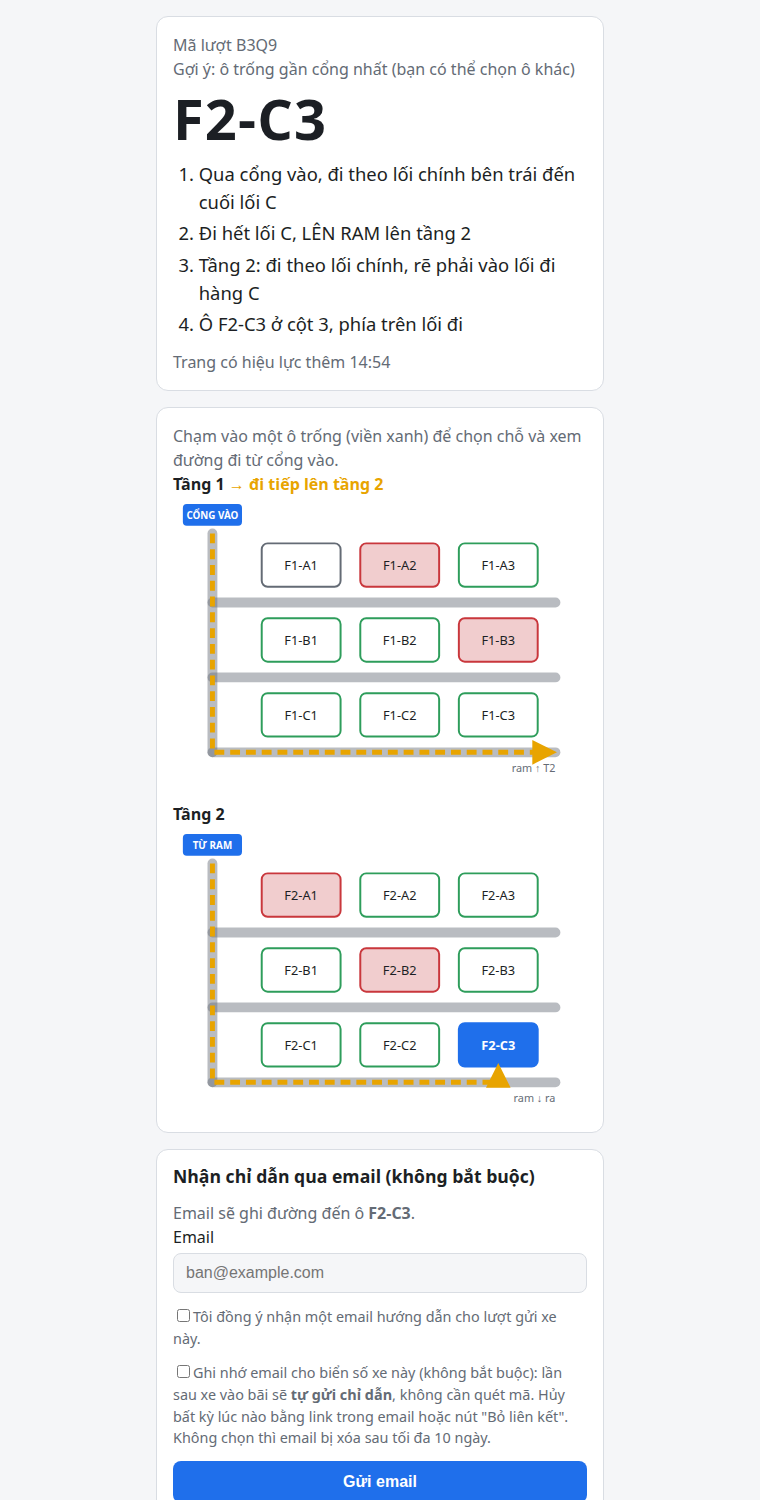
\includegraphics[width=0.5\textwidth]{hinh/web-qr-duongdi.png}
\caption{Trang của khách: gợi ý ô F2-C3, đường đi lên tầng 2 và ô nhập email (chạy với dữ liệu mẫu)}
\label{fig:qr}
\end{figure}

\section{Kiểm thử với camera thật}\label{sec:camthat}

Camera OV5647 trên Pi 5, hai vùng làn là hai nửa khung hình. Kết quả quan sát:
\begin{itemize}
  \item Làn trống: tỉ lệ khác nền gần 0\,\% ở cả hai làn, không gửi sự kiện nhầm.
  \item Đưa tay vào làn: tỉ lệ khác nền vượt ngưỡng 8\,\%, khung làn đổi màu, gửi \emph{đúng một} sự kiện cho mỗi lần đưa tay. Giữ tay lâu không tạo thêm lượt.
  \item Đổi góc camera: bấm \emph{Chụp lại nền} khi làn trống thì phát hiện chạy lại bình thường.
\end{itemize}
Có lần camera chỉ gửi được một khung hình rồi treo, do cáp camera cắm lỏng; cắm lại thì chạy bình thường. Nút \emph{Thử xe VÀO}, \emph{Thử xe RA} trên trang camera gửi đúng loại tin nhắn như camera, nên cũng dùng được để kiểm tra phần còn lại của hệ thống.

\section{Bảng nghiệm thu theo kịch bản}

\begin{longtable}{@{}P{1.3cm}P{7.4cm}P{3.1cm}P{2.3cm}@{}}
\caption{Kết quả nghiệm thu SIM-01 đến SIM-16}\label{tab:nghiemthu}\\
\toprule
\textbf{Mã} & \textbf{Kịch bản} & \textbf{Kiểm bằng} & \textbf{Kết quả} \\ \midrule
\endfirsthead
\toprule
\textbf{Mã} & \textbf{Kịch bản} & \textbf{Kiểm bằng} & \textbf{Kết quả} \\ \midrule
\endhead
SIM-01 & Đưa tay vào làn vào: một phiên chờ cho vào, biển 11111, cần chưa mở & Mức 1, mức 4 & Đạt \\
SIM-02 & Nhân viên \emph{Cho vào}: cần quay trái rồi về giữa, xe vào danh sách (web và Pi), màn hình ở cổng có QR & Mức 1, mức 4 & Đạt \\
SIM-03 & Chọn ô tầng 2 trên trang QR, nhập email: đường đi lên dốc; một email đúng ô & Mức 1, mức 3 & Đạt \\
SIM-04 & Ghi nhớ email: lần sau tự gửi; hủy liên kết thì không gửi & Mức 1, mức 3 & Đạt \\
SIM-05 & Nút ô đảo trạng thái, giữ được sau khi khởi động lại, không đổi phiên đỗ & Bo mạch thật & Đạt \\
SIM-06 & Bãi đầy: không cho vào, không mở cần & Mức 1 & Đạt \\
SIM-07 & Xe ra: chọn xe số lớn nhất, hiện số tiền; chỉ mở cần khi nhân viên cho ra (có phí thì sau khi thu); xe rời danh sách & Mức 1, mức 4 & Đạt \\
SIM-08 & Giữ tay lâu, rút ra đưa lại: mỗi lần đưa tay đúng một lượt & Mức 2, mức 4 & Đạt \\
SIM-09 & Hai lượt chờ vào nhận biển khác nhau; từ chối một lượt thì số được dùng lại & Mức 1 & Đạt \\
SIM-10 & Gửi lặp cùng mã sự kiện, mã lệnh & Mức 1, mô phỏng cổng & Đạt \\
SIM-11 & Bo mạch ô mất kết nối quá 90 giây: ô thành không rõ, xe vẫn được cho vào & Mức 1 & Đạt \\
SIM-12 & Lệnh cũ gửi tới sau khi cổng kết nối lại bị bỏ qua & Mô phỏng cổng & Đạt \\
SIM-13 & Camera báo xe ra khi bãi trống: bỏ qua & Mức 1 & Đạt \\
SIM-14 & SES gửi lỗi: vẫn chỉ đường, ghi gửi thất bại & Mức 1 & Đạt \\
SIM-15 & Link sai hoặc hết hạn, gửi email lần hai & Mức 1 & Đạt \\
SIM-16 & Dữ liệu định danh quá 10 ngày bị ẩn và xóa & Mức 1, chạy tác vụ trên AWS & Đạt \\
\bottomrule
\end{longtable}

\section{Đánh giá}

\subsection{Mức đáp ứng yêu cầu}

Luồng chính chạy được trên AWS với thiết bị thật: xe vào (chờ cho vào, nhân viên cho vào), chỉ đường, xe ra (chờ cho ra, thu tiền, cho ra). Cả 16/16 kịch bản nghiệm thu đều đạt.

\subsection{Số liệu đo}

\begin{table}[H]
\centering
\caption{Số liệu đo trên hệ thống thật}
\label{tab:solieu}
\begin{tabularx}{\textwidth}{@{}LP{5.6cm}@{}}
\toprule
\textbf{Chỉ số} & \textbf{Kết quả} \\ \midrule
Thời gian từ lúc gửi sự kiện có xe tới khi đám mây xử lý xong (10 lần đo ngày 27/11/2026, gửi từ laptop ở Hà Nội tới vùng Singapore) & Trung vị 0,22 giây; nhỏ nhất 0,20 giây; lớn nhất 1,99 giây (lần đầu, Lambda khởi động nguội) \\
Số kịch bản nghiệm thu đạt & 16/16 \\
Số kiểm thử tự động đạt & 16/16 (đám mây), 5/5 (Pi) \\
Chi phí AWS thực tế từ 1/11 đến 27/11/2026 (theo AWS Cost Explorer) & Khoảng 0,09 USD, đã được tín dụng trừ hết. Nhiều nhất là DynamoDB (0,046 USD) và API Gateway (0,016 USD) \\
\bottomrule
\end{tabularx}
\end{table}

Thời gian xử lý đáp ứng NFR-07 (dưới 2 giây). Chi phí thực tế thấp hơn nhiều so với ước tính ở Bảng~\ref{tab:chiphi}, vì hệ thống chỉ chạy vài giờ mỗi ngày để làm demo.

\subsection{Hạn chế}

\begin{itemize}
  \item Camera chỉ phát hiện ``có vật'' trong làn, không đọc biển số. Biển số là số demo do hệ thống cấp. Xe ra luôn là xe có số lớn nhất, nhân viên không chọn được xe khác.
  \item Biển số demo được dùng lại cho xe sau. Vì vậy email đã ghi nhớ theo một biển demo sẽ được gửi cho lượt sau; cần bỏ liên kết sau khi demo.
  \item 18 ô dùng nút nhấn giả lập cảm biến, chưa chứng minh được việc phát hiện xe thật. Bãi đầy chỉ tính theo nút ô.
  \item Không có cảm biến xe qua cổng, nên mọi lượt vào, ra cần nhân viên bấm cho phép.
  \item SES đang ở chế độ thử, chỉ gửi được tới địa chỉ đã xác minh.
\end{itemize}

\chapter{Bàn giao}

Mục tiêu của bước này là để người vận hành bãi tự dùng được hệ thống: biết khởi động, theo dõi, xử lý các tình huống hay gặp, cập nhật và gỡ bỏ toàn bộ hạ tầng khi cần.

\section{Danh mục bàn giao}\label{sec:danhmuc}

\begin{longtable}{@{}P{3.6cm}P{7.2cm}P{3.3cm}@{}}
\caption{Danh mục bàn giao}\label{tab:bangiao}\\
\toprule
\textbf{Hạng mục} & \textbf{Nội dung} & \textbf{Hình thức} \\ \midrule
\endfirsthead
\toprule
\textbf{Hạng mục} & \textbf{Nội dung} & \textbf{Hình thức} \\ \midrule
\endhead
Mã nguồn & Phần đám mây, web, chương trình trên Pi, phần mềm ESP32, chương trình mô phỏng, kiểm thử & Kho GitHub (nhánh \code{main}) \\
Hạ tầng dưới dạng mã & \code{template.yaml} và 7 script triển khai, gỡ bỏ & Thư mục \code{infra/aws/} \\
Tài liệu kỹ thuật & Kiến trúc, tình huống sử dụng, sơ đồ bãi, quy ước tin nhắn và API, phần cứng, kế hoạch kiểm thử & Thư mục \code{docs/} \\
Hướng dẫn cài đặt & Từng bước từ cấu hình AWS CLI tới nạp phần mềm ESP32 & \code{docs/\allowbreak{}setup-guide.md} \\
Tài khoản ứng dụng & \code{admin} (ADMIN) và \code{kiosk} (KIOSK) trên Cognito & Giao trực tiếp; người nhận đặt mật khẩu mới bằng \code{create-users.sh} \\
Chứng chỉ thiết bị & 3 bộ chứng chỉ và khóa riêng (\code{pi-01}, \code{gate-01}, \code{slots-01}) & Thư mục \code{secrets/}, chép qua kênh an toàn, không gửi qua email hay kho mã \\
Cấu hình triển khai & Email gửi SES, email nhận cảnh báo chi phí, khóa ký QR & \code{secrets/\allowbreak{}deploy.env} \\
Thiết bị & Pi đã cài chương trình phát hiện xe; ESP32-S3 (cần chắn hai hướng) và ESP32 (18 nút) đã nạp phần mềm & Tại chỗ \\
\bottomrule
\end{longtable}

\section{Hướng dẫn vận hành}

\subsection{Khởi động hằng ngày}

\begin{lenh}
# Trên Pi: dịch vụ pi-vision tự chạy khi bật nguồn
journalctl -u pi-vision -n 30 --no-pager | grep MQTT
#   -> phải có dòng "Đã kết nối MQTT"

# Cắm điện ESP32-S3 (servo có nguồn 5 V riêng, nối chung GND)
# và ESP32 18 nút; cả hai tự vào Wi-Fi đã khai báo
\end{lenh}

Sau đó mở \code{/admin}, thẻ \emph{Tổng quan}: cả \code{pi-01}, \code{gate-01}, \code{slots-01} phải ở trạng thái ONLINE. Mở \code{/kiosk} trên màn hình ở cổng, \code{/admin/\allowbreak{}sessions} trên máy của nhân viên, và trang camera \code{http:/\allowbreak{}/\allowbreak{}<ip-pi>:8000} nếu cần.

\subsection{Tình huống hay gặp}

\begin{longtable}{@{}P{4.6cm}P{9.5cm}@{}}
\caption{Xử lý tình huống khi vận hành}\label{tab:runbook}\\
\toprule
\textbf{Tình huống} & \textbf{Cách xử lý} \\ \midrule
\endfirsthead
\toprule
\textbf{Tình huống} & \textbf{Cách xử lý} \\ \midrule
\endhead
Có xe ở làn vào & Vào \emph{Phiên đỗ}, thẻ ``Chờ cho vào'' hiện biển số. Bấm \emph{Cho vào} để mở cần. Nếu camera báo nhầm thì bấm \emph{Không cho vào}. Mọi thao tác đều được ghi lại người thực hiện. \\
Có xe ở làn ra & Thẻ ``Chờ cho ra'' hiện số tiền. Miễn phí thì bấm \emph{Cho ra}. Có phí thì thu tiền mặt rồi bấm \emph{Đã thu \ldots{} cho ra}, hoặc bấm \emph{Miễn phí} và ghi lý do. Xe rời danh sách ngay. \\
Khách muốn hủy email tự gửi & Khách bấm \emph{Hủy liên kết} trong email, hoặc \emph{Bỏ liên kết email} trên trang QR. \\
Thiết bị mất kết nối & Kiểm tra nguồn và Wi-Fi. Với Pi, xem \code{systemctl status pi-vision}. Nếu mạng chặn cổng 8883 thì đặt \code{port = 443} trong \code{config.local.toml} và khởi động lại dịch vụ. \\
Ô hiện ``không rõ'' & Bo mạch ô mất kết nối quá 90 giây. Ô tự trở lại khi bo mạch gửi trạng thái. \\
Bấm cho vào, cho ra mà cần không quay & Xem cảnh báo ở \emph{Tổng quan}. Xem log của ESP32-S3: nếu có dòng ra lệnh servo mà servo không quay thì servo đang thiếu nguồn 5~V. Có thể mở cần bằng tay (hệ thống ghi cảnh báo). \\
Camera báo nhầm hoặc không nhận tay & Trên trang camera: bỏ tay ra rồi bấm \emph{Chụp lại nền}. Chỉnh vùng làn và độ nhạy trong \code{config.toml}. Lượt báo nhầm thì bấm \emph{Không cho vào}. \\
Trang camera báo ``không có hình'' & Tắt Pi, cắm lại cáp camera cho chặt, kiểm tra nguồn. Trong lúc đó vẫn dùng được nút \emph{Thử xe VÀO}, \emph{Thử xe RA}. \\
Đổi bảng giá & Vào \emph{Bảng giá}. Phiên đỗ đang mở vẫn giữ bảng giá lúc vào. \\
Nhận email cảnh báo chi phí & Kiểm tra trang Billing; nếu không dùng nữa thì gỡ hạ tầng (mục~\ref{sec:gobo}). \\
\bottomrule
\end{longtable}

\subsection{Cập nhật và bảo trì}

\begin{itemize}
  \item Cập nhật phần đám mây: chạy \code{git pull}, rồi chạy lại \code{deploy.sh} trong \code{infra/\allowbreak{}aws}. CloudFormation chỉ đổi phần thay đổi.
  \item Cập nhật web: chạy \code{infra/\allowbreak{}aws/\allowbreak{}deploy-web.sh}.
  \item Cập nhật Pi: chạy \code{git pull} trong \code{\textasciitilde/\allowbreak{}Cloud-Course}, chạy lại \code{install-pi.sh}, rồi khởi động lại dịch vụ \code{pi-vision}.
  \item Thêm tài khoản: tạo người dùng Cognito và thêm vào nhóm ADMIN hoặc KIOSK (\code{create-users.sh} là mẫu).
  \item Thiết bị bị mất: vô hiệu hóa chứng chỉ của thiết bị đó trong IoT Core, rồi chạy lại \code{provision-devices.sh} để cấp chứng chỉ mới.
  \item Xem log: trên Pi dùng \code{journalctl -u pi-vision}; với Lambda dùng \code{aws logs tail /\allowbreak{}aws/\allowbreak{}lambda/\allowbreak{}smart-parking-dev-iot --follow}.
\end{itemize}

\subsection{Tắt an toàn}

Với Pi: chạy \code{sudo shutdown -h now} hoặc nhấn nút nguồn một lần. Chờ đèn chuyển đỏ mới rút điện. Hạ tầng AWS có thể để nguyên: khi không có thiết bị gửi tin, chi phí gần như bằng không.

\subsection{Gỡ bỏ toàn bộ hạ tầng}\label{sec:gobo}

\begin{lenh}
cd infra/aws && ./destroy.sh   # xóa web, stack, Thing, chứng chỉ, chính sách
\end{lenh}

\section{Hướng dẫn sử dụng theo vai trò}\label{sec:huongdan}

\begin{table}[H]
\centering
\caption{Nội dung hướng dẫn theo vai trò}
\label{tab:daotao}
\begin{tabularx}{\textwidth}{@{}P{3.4cm}LP{1.8cm}@{}}
\toprule
\textbf{Đối tượng} & \textbf{Nội dung} & \textbf{Thời lượng} \\ \midrule
Nhân viên bãi & Đăng nhập; đọc trang Tổng quan và danh sách xe; \emph{Cho vào}, \emph{Không cho vào}; thu tiền, miễn phí, \emph{Cho ra}; mở cần bằng tay; sửa bảng giá & 1 buổi \\
Kỹ thuật viên thiết bị & Khởi động thiết bị; chỉnh vùng làn và độ nhạy; nối mạng cho Pi qua dây LAN; xem log; đổi Wi-Fi và nạp phần mềm ESP32; cấp nguồn cho servo & 1 buổi \\
Người phụ trách hệ thống & Cấu trúc kho mã; AWS CLI; triển khai, cập nhật, gỡ hạ tầng; cấp và thu hồi chứng chỉ; đọc log CloudWatch; theo dõi chi phí & 1 buổi \\
\bottomrule
\end{tabularx}
\end{table}

Sau buổi hướng dẫn, người học tự làm lại một vòng xe vào, xe ra và một lần triển khai lại hạ tầng.

\section{Bảng kiểm nghiệm thu}\label{sec:bienban}

Bảng~\ref{tab:kiemnghiemthu} đối chiếu tiêu chí nghiệm thu (mục~\ref{sec:nghiemthu}) với kết quả kiểm thử ở Chương~6.

\begin{table}[H]
\centering
\caption{Bảng kiểm nghiệm thu}
\label{tab:kiemnghiemthu}
\begin{tabularx}{\textwidth}{@{}LP{2.2cm}P{3.6cm}@{}}
\toprule
\textbf{Hạng mục} & \textbf{Kết quả} & \textbf{Căn cứ} \\ \midrule
Xe vào (cho vào), chỉ đường, xe ra (thu tiền, cho ra) chạy trên AWS & $\checkmark$ Đạt & SIM-01, 02, 07; mục~\ref{sec:vong2} \\
Màn hình QR ở cổng, trang khách (chọn ô, bản đồ đường đi), email và ghi nhớ email & $\checkmark$ Đạt & SIM-03, 04, 14, 15 \\
Trang quản trị: danh sách xe, cho vào, cho ra, thu tiền, bảng giá, thiết bị, cảnh báo & $\checkmark$ Đạt & SIM-02, 06, 07 \\
Camera phát hiện xe ở hai làn; một cần quay đúng hai hướng; 18 nút báo đúng ô & $\checkmark$ Đạt & SIM-05, 08; mục~\ref{sec:camthat} \\
Bảo mật thiết bị, phân quyền người dùng, xóa dữ liệu sau 10 ngày & $\checkmark$ Đạt & Kiểm thử \code{permissions}, SIM-16 \\
Dựng và gỡ hạ tầng bằng script & $\checkmark$ Đạt & Mục~\ref{sec:trienkhaicloud} \\
Tài liệu và hướng dẫn sử dụng & $\checkmark$ Đạt & Mục~\ref{sec:danhmuc} đến~\ref{sec:huongdan} \\
\bottomrule
\end{tabularx}
\end{table}

\chapter{Kết luận}

\section{Kết quả đạt được}

Nhóm đã đi đủ các bước của một dự án đưa ứng dụng lên đám mây, từ nhận yêu cầu đến bàn giao:

\begin{itemize}
  \item Phân tích và lập kế hoạch. Từ 6 mục tiêu và 11 vấn đề cần làm rõ, nhóm xác định 13 yêu cầu chức năng và 10 yêu cầu phi chức năng. Nhóm so sánh các phương án (AWS hay OpenStack, không máy chủ hay máy ảo, xử lý ảnh tại bãi hay trên đám mây), và ước tính chi phí khoảng 3--5 USD mỗi tháng.
  \item Thiết kế. Kiến trúc không máy chủ trên AWS với IoT Core, Lambda, DynamoDB, API Gateway, Cognito, SES, S3, CloudFront, EventBridge, CloudWatch và Budgets. Thiết bị, web và đám mây giao tiếp theo hai quy ước cố định. Cho xe vào bằng một giao dịch không bị chia cắt. Nhân viên cho phép từng lượt vào, ra. Trang khách gợi ý ô và vẽ đường đi. Khách tự chọn có ghi nhớ email hay không. Dữ liệu cá nhân bị xóa sau 10 ngày.
  \item Triển khai. Toàn bộ hạ tầng dựng bằng một template CloudFormation và các script AWS CLI. Pi 5 có camera kết nối AWS. ESP32-S3 điều khiển một cần chắn hai hướng, ESP32 đọc 18 nút giả lập cảm biến ô; cả hai đều đã nạp phần mềm và chạy với AWS.
  \item Kiểm thử. 16/16 kiểm thử nghiệp vụ và 5/5 kiểm thử phần phát hiện xe đạt. Luồng vào, chỉ đường, ra chạy được trên AWS với thiết bị thật. 16/16 kịch bản nghiệm thu đạt. Thời gian xử lý một sự kiện có trung vị 0,22 giây. Chi phí thực tế cả tháng khoảng 0,09 USD.
  \item Bàn giao. Mã nguồn, hạ tầng dưới dạng mã, tài liệu kỹ thuật, hướng dẫn cài đặt và vận hành, nội dung hướng dẫn theo vai trò và bảng kiểm nghiệm thu.
\end{itemize}

Qua đề tài, nhóm rút ra một số bài học:
\begin{itemize}
  \item Chốt sớm quy ước giao tiếp giúp các phần thiết bị, đám mây và web làm song song được, nhờ có chương trình mô phỏng.
  \item Hạ tầng dưới dạng mã giúp dựng lại và gỡ bỏ an toàn. Tệp template cũng là tài liệu chính xác nhất về hệ thống.
  \item Nắm rõ thiết bị sẵn có (phiên bản Python của Pi, mạng chặn cổng, nguồn cho servo) giúp thấy sớm những rủi ro chỉ lộ ra khi lắp thật.
  \item Chạy thử sớm với thiết bị thật giúp phát hiện các lỗi chỉ xuất hiện khi lắp thật, như nguồn cho servo hay cáp camera cắm lỏng.
  \item Kiểm thử tự động cần phủ cả các tác vụ chạy ngầm. Một lỗi xóa nhầm hàm dọn dữ liệu chỉ được phát hiện khi thêm kiểm thử cho tác vụ này.
\end{itemize}

\begin{thebibliography}{99}
\addcontentsline{toc}{chapter}{Tài liệu tham khảo}
\setlength{\itemsep}{2pt}
\small
\bibitem{iotmqtt} Amazon Web Services, \emph{AWS IoT Core Developer Guide --- MQTT}. \url{https://docs.aws.amazon.com/iot/latest/developerguide/mqtt.html}
\bibitem{iotpolicy} Amazon Web Services, \emph{AWS IoT Core policies}. \url{https://docs.aws.amazon.com/iot/latest/developerguide/iot-policies.html}
\bibitem{iotalpn} Amazon Web Services, \emph{Device communication protocols (MQTT over port 443 with ALPN)}. \url{https://docs.aws.amazon.com/iot/latest/developerguide/protocols.html}
\bibitem{iotrules} Amazon Web Services, \emph{Rules for AWS IoT}. \url{https://docs.aws.amazon.com/iot/latest/developerguide/iot-rules.html}
\bibitem{lambda} Amazon Web Services, \emph{AWS Lambda Developer Guide}. \url{https://docs.aws.amazon.com/lambda/latest/dg/welcome.html}
\bibitem{ddbtx} Amazon Web Services, \emph{Amazon DynamoDB Transactions}. \url{https://docs.aws.amazon.com/amazondynamodb/latest/developerguide/transactions.html}
\bibitem{ddbttl} Amazon Web Services, \emph{Using Time to Live (TTL) in DynamoDB}. \url{https://docs.aws.amazon.com/amazondynamodb/latest/developerguide/TTL.html}
\bibitem{apigw} Amazon Web Services, \emph{Controlling access to HTTP APIs with JWT authorizers}. \url{https://docs.aws.amazon.com/apigateway/latest/developerguide/http-api-jwt-authorizer.html}
\bibitem{cognito} Amazon Web Services, \emph{Amazon Cognito user pools}. \url{https://docs.aws.amazon.com/cognito/latest/developerguide/cognito-user-pools.html}
\bibitem{ses} Amazon Web Services, \emph{Amazon SES --- Request production access (moving out of the sandbox)}. \url{https://docs.aws.amazon.com/ses/latest/dg/request-production-access.html}
\bibitem{oac} Amazon Web Services, \emph{Restricting access to an Amazon S3 origin (Origin Access Control)}. \url{https://docs.aws.amazon.com/AmazonCloudFront/latest/DeveloperGuide/private-content-restricting-access-to-s3.html}
\bibitem{cfnpkg} Amazon Web Services, \emph{AWS CLI Command Reference --- cloudformation package}. \url{https://docs.aws.amazon.com/cli/latest/reference/cloudformation/package.html}
\bibitem{sam} Amazon Web Services, \emph{AWS Serverless Application Model (SAM) Specification}. \url{https://docs.aws.amazon.com/serverless-application-model/}
\bibitem{pricing} Amazon Web Services, \emph{AWS Pricing Calculator}. \url{https://calculator.aws/}
\bibitem{wellarch} Amazon Web Services, \emph{AWS Well-Architected Framework}. \url{https://docs.aws.amazon.com/wellarchitected/latest/framework/welcome.html}
\bibitem{picam} Raspberry Pi Ltd, \emph{The Picamera2 Library}. \url{https://datasheets.raspberrypi.com/camera/picamera2-manual.pdf}
\bibitem{mqttspec} OASIS, \emph{MQTT Version 3.1.1}. \url{https://docs.oasis-open.org/mqtt/mqtt/v3.1.1/mqtt-v3.1.1.html}
\bibitem{repo} Mã nguồn đề tài. \url{https://github.com/Tuyen230605/Smart_parking}
\end{thebibliography}

\appendix
\renewcommand{\thechapter}{\Alph{chapter}}
\titleformat{\chapter}[display]{\bfseries\Large\centering}{PHỤ LỤC \thechapter}{6pt}{\Large\MakeUppercase}

\chapter{Trình tự lệnh triển khai đầy đủ}

\begin{lenh}
# -- Laptop: làm một lần ----------------------------------------
aws configure                 # vùng ap-southeast-1, định dạng json
aws sts get-caller-identity
git clone https://github.com/Tuyen230605/Smart_parking.git
cd Smart_parking
python3 -m venv .venv
.venv/bin/pip install -r simulation/requirements.txt pytest "moto[dynamodb]"

cd infra/aws
./deploy.sh                   # hạ tầng + 18 ô + bảng giá
./create-users.sh             # tài khoản admin, kiosk
WIFI_SSID=<wifi> WIFI_PASS=<mật khẩu> ./provision-devices.sh
./deploy-web.sh               # web lên S3 + CloudFront
./setup-pi.sh oi@<ip-pi>      # mã + chứng chỉ + cài đặt trên Pi

# -- Pi ------------------------------------------------------------
cd ~/Cloud-Course/edge/raspberry-pi-vision
journalctl -u pi-vision -f

# -- ESP32 (mỗi bo mạch một lần) -----------------------------------
cd firmware/esp32-gates && pio run -t upload
cd firmware/esp32-slot-sensors && pio run -t upload

# -- Kiểm thử ------------------------------------------------------
cd backend && ../.venv/bin/python -m pytest -q tests

# -- Kết thúc đồ án ------------------------------------------------
cd infra/aws && ./destroy.sh
\end{lenh}

\chapter{Ví dụ tin nhắn MQTT}

Lệnh mở cần (đám mây gửi ESP32):
\begin{lenh}
{"schema_version": 1, "message_type": "gate_command",
 "command_id": "6ff2b85d-50bc-4ea4-94bd-5f3430d4cf55",
 "target_device_id": "gate-01", "gate": "ENTRY", "action": "OPEN",
 "session_id": "01J9F7VRW8MW6W1MJZCQNNMJZP",
 "issued_at": "2026-11-25T09:00:02Z",
 "expires_at": "2026-11-25T09:00:07Z"}
\end{lenh}

Phản hồi của cổng (ESP32 gửi đám mây):
\begin{lenh}
{"schema_version": 1, "message_type": "gate_telemetry",
 "event_id": "c9ff7d15-b9fb-4318-8b5f-33989d5dd130",
 "device_id": "gate-01",
 "command_id": "6ff2b85d-50bc-4ea4-94bd-5f3430d4cf55",
 "gate": "ENTRY", "state": "OPEN", "error_code": null,
 "occurred_at": "2026-11-25T09:00:03Z"}
\end{lenh}

Trạng thái ô (một ô thay đổi):
\begin{lenh}
{"schema_version": 1, "message_type": "slot_changed",
 "event_id": "af3cdb82-213e-4df2-9182-e13d08767231",
 "device_id": "slots-01", "boot_id": "91270fd2-...", "seq": 101,
 "occurred_at": "2026-11-25T09:01:00Z",
 "slot_id": "F1-A1", "occupied": true, "source": "BUTTON"}
\end{lenh}

Danh sách xe (đám mây gửi Pi, kênh \code{vision/\allowbreak{}pi-01/\allowbreak{}lot}):
\begin{lenh}
{"schema_version": 1, "message_type": "lot_state",
 "occurred_at": "2026-11-25T09:45:41.753Z",
 "in_lot": ["11111", "22222"],
 "pending_entry": ["33333"], "pending_exit": []}
\end{lenh}

\chapter{Chính sách IoT của thiết bị \code{pi-01}}

Đây là ví dụ quyền tối thiểu. Pi chỉ được kết nối bằng đúng tên của mình, chỉ được gửi vào hai kênh của mình và chỉ được nhận kênh danh sách xe. Pi không nhận được lệnh mở cần và không đọc được kênh của thiết bị khác. Trong đoạn dưới, \code{A} là viết tắt của \code{arn:aws:iot:ap-southeast-1:<mã tài khoản>}, và \code{T} là viết tắt của \code{parking/v1/site-01}.

\begin{lenh}
{"Version": "2012-10-17", "Statement": [
  {"Effect": "Allow", "Action": "iot:Connect",
   "Resource": "A:client/pi-01"},
  {"Effect": "Allow", "Action": "iot:Publish",
   "Resource": ["A:topic/T/vision/pi-01/events",
                "A:topic/T/devices/pi-01/status"]},
  {"Effect": "Allow", "Action": "iot:Subscribe",
   "Resource": "A:topicfilter/T/vision/pi-01/lot"},
  {"Effect": "Allow", "Action": "iot:Receive",
   "Resource": "A:topic/T/vision/pi-01/lot"}]}
\end{lenh}


\end{document}
